\section{Robot (Imitation) Learning}
\label{sec:learning-imitation}

\epigraph{\emph{The best material model for a cat is another, or preferably the same cat}}{Norbert Wiener}

\begin{tldr}
Behavioral Cloning provides a natural platform to learn from real-world interactions without the need to design any reward function, and generative models prove more effective than point-wise policies at dealing with multimodal demonstration datasets.
\end{tldr}

% \paragraph{A Change in Notation}
% The reinforcement learning and generative modeling communities have developed largely in parallel, leading to notable differences in notation. To keep this tutorial approachable as an entry point to both literatures, we follow the conventions commonly used within each field. As a result, some symbols may appear with more than one meaning. Table~\ref{tab:notation-change} summarizes these cases and provides disambiguation.

% \begin{table}
    \centering
    \begin{tabular}{ccc}
                     & \textbf{Reinforcement Learning} & \textbf{Behavioral Cloning}  \\
    \rowcolor[HTML]{EFEFEF} 
    \( \mathcal D \) & Environment dynamics            & Finite set of demonstrations \\
    \( \mathbb P \)  & Probability (general)           & (unused)                     \\
    \rowcolor[HTML]{EFEFEF} 
    \( p, q \) & (unused) & \begin{tabular}[c]{@{}c@{}}Probability, according to\\ a given distribution (different\\ between \( p \) and \( q \))\end{tabular} \\
                     &                                 &                             
    \end{tabular}
    \caption{Changes in notation between the Reinforcement Learning and Behavioral Cloning frameworks.}
    \label{tab:notation-change}
\end{table}

\begin{figure}
    \centering
    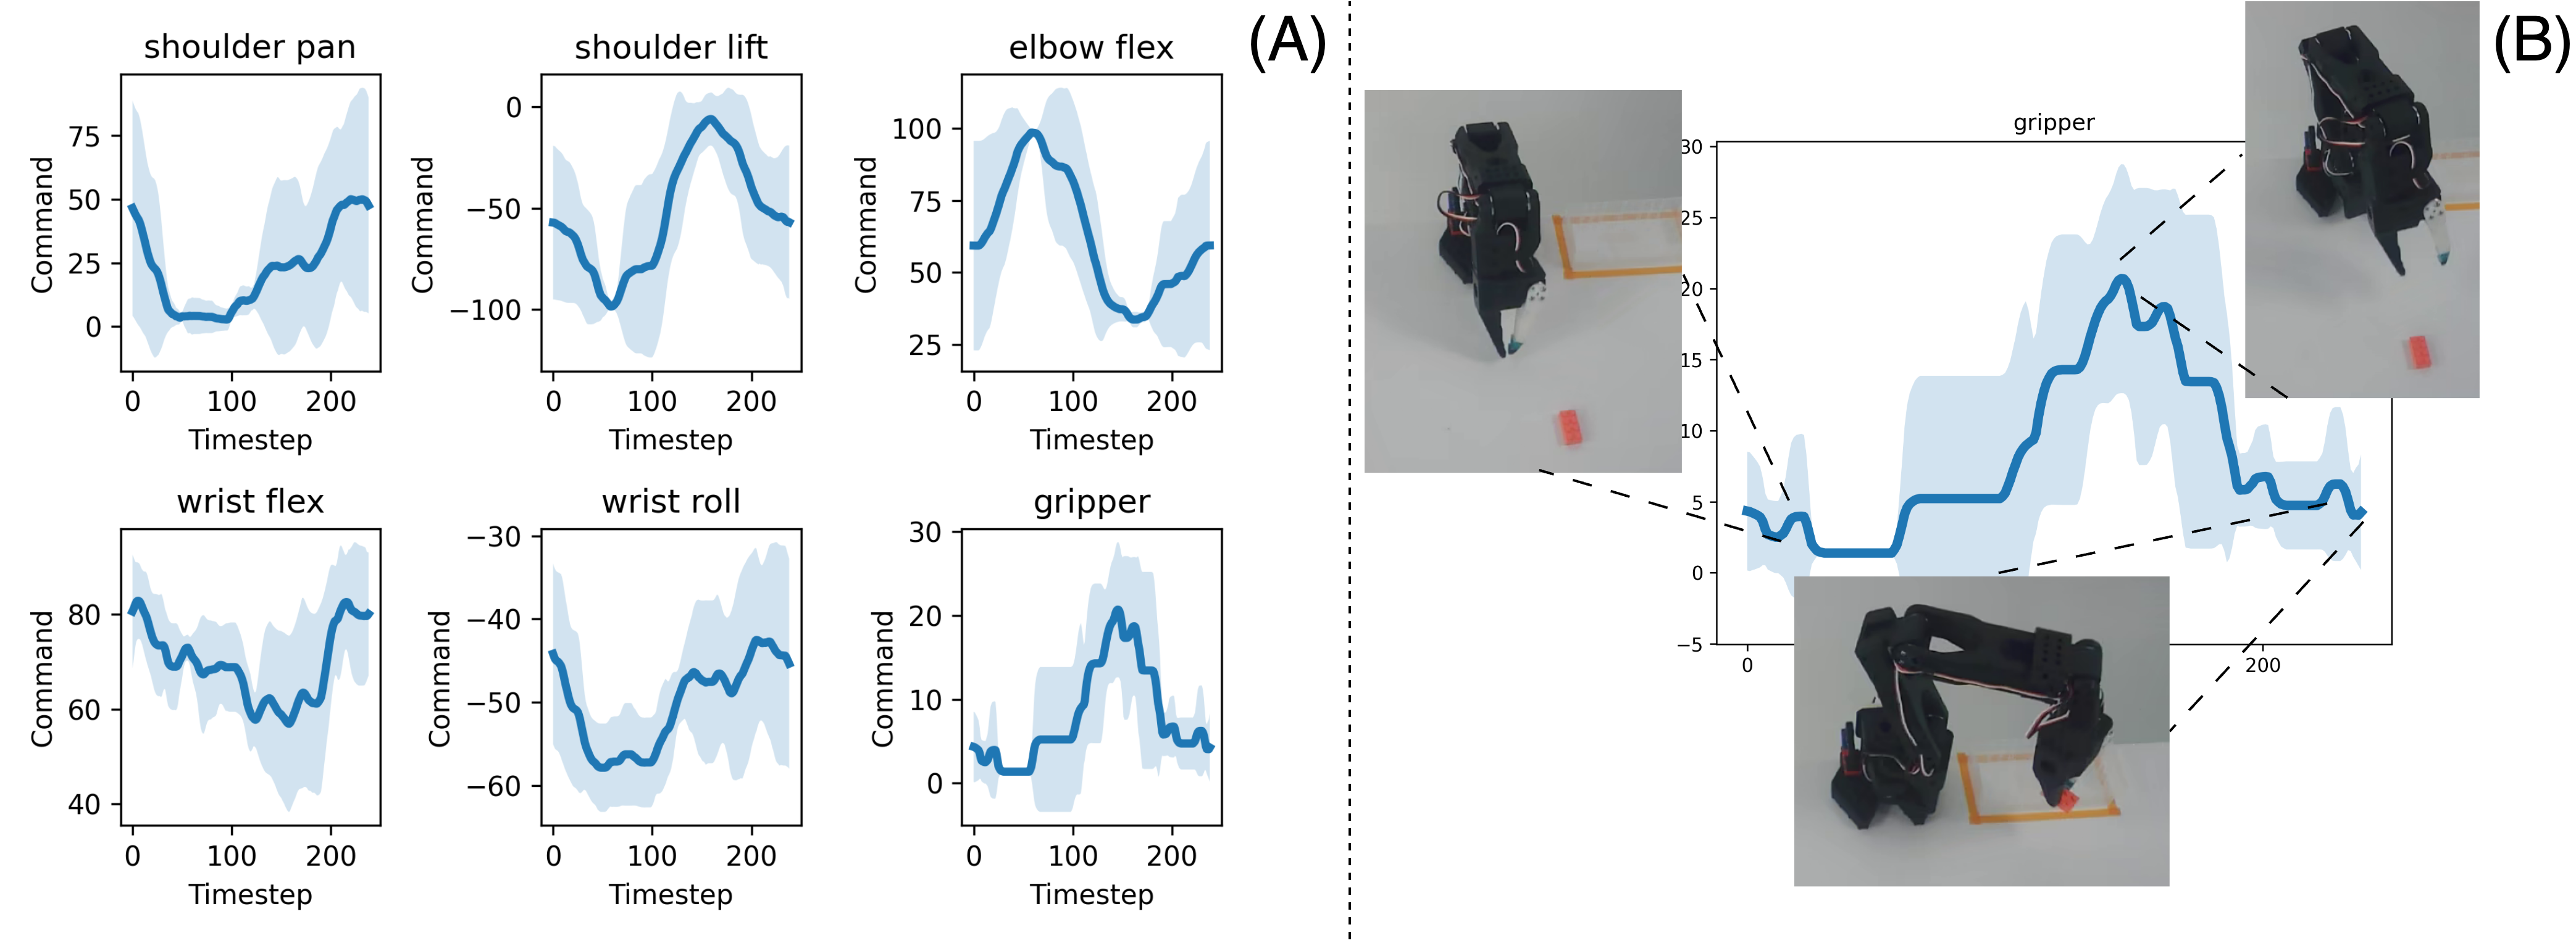
\includegraphics[width=0.8\textwidth]{figures/ch4/ch4-bc-trajectories.png}
    \caption{(A) Average (with standard deviation) evolution of the actuation levels over the first 5 recorded episodes in \url{lerobot/svla_so101_pickplace}. Proprioperceptive states provide invaluable to determine the robot's state during an episode. (B) Camera frames are also recorded alongside measurements on the robot's state, capturing information about the robot's interaction with its environment.}
    \label{fig:ch4-bc-trajectories}
\end{figure}

Learning from human demonstrations provides a pragmatic alternative to the RL pipeline discussed in Section~\ref{sec:learning-rl}.
Indeed, especially in real-world robotics, online exploration is typically \highlight{costly and potentially unsafe}, and designing (dense) reward signals is a \highlight{brittle and task-specific} process.
Further, even success detection itself often requires bespoke instrumentation, while episodic training demands reliable resets---all factors complicating training RL algorithms on hardware at scale.
Behavioral Cloning (BC) sidesteps these constraints by \highlight{casting control an imitation learning problem}, leveraging previously collected expert demonstrations to anchor the learned autonomous behavior.
Most notably, by \emph{learning-to-imitate}, autonomous systems naturally adhere to the objectives, preferences, and success criteria implicitly encoded in the data, which reduces early-stage exploratory failures and obviates hand-crafted reward shaping altogether.

Formally, let \( \mathcal D = \{ \tau^{(i)} \}_{i=1}^N \) be a set of expert trajectories, with \( \tau^{(i)} = \{(o_t^{(i)}, a_t^{(i)})\}_{t=0}^{T_i} \) representing the \(i\)-th length-\(T_i\) trajectory in \( \mathcal D \), \(o_t \in \obsspace \) denoting observations (e.g., images and proprioception altogether), and \(a_t \in \actionspace \) the expert actions.
Typically, observations \( o \in \obsspace \) consist of both image and proprioperceptive information, while actions \( a \in \actionspace \) represent control specifications for the robot to execute, e.g. a joint configuration.
Note that differently from Section~\ref{sec:learning-rl}, in the imitation learning context \( \mathcal D \) denotes an offline dataset collecting \( N \) length-\( T_i \) reward-free (expert) human trajectories \( \tau^{(i)} \), and \emph{not} the environment dynamics.
Similarily, in this section \( \tau^{(i)} \) represent a length-\(T_i\) trajectory of observation-action pairs, which crucially \emph{omits entirely any reward} information.
Figure~\ref{fig:ch4-bc-trajectories} graphically shows trajectories in terms of the average evolution of the actuation on the 6 joints of a teleoperated SO-100 manipulator.
Notice how proprioperceptive states are captured jointly with camera frames over the course of the recorded episodes, providing a unified high-frame rate collection of both image and joint teleoperation data.
Figure~\ref{fig:ch4-observation-action-mapping} shows \( (o_t, a_t) \)-pairs for the same dataset, with the actions performed by the human expert illustrated alongside the corresponding observation.
In principle, (expert) trajectories \( \tau^{(i)} \) can have different lengths since demonstrations might exhibit multi-modal strategies to attain the same goal, resulting in multiple, different behaviors.


\begin{figure}
    \centering
    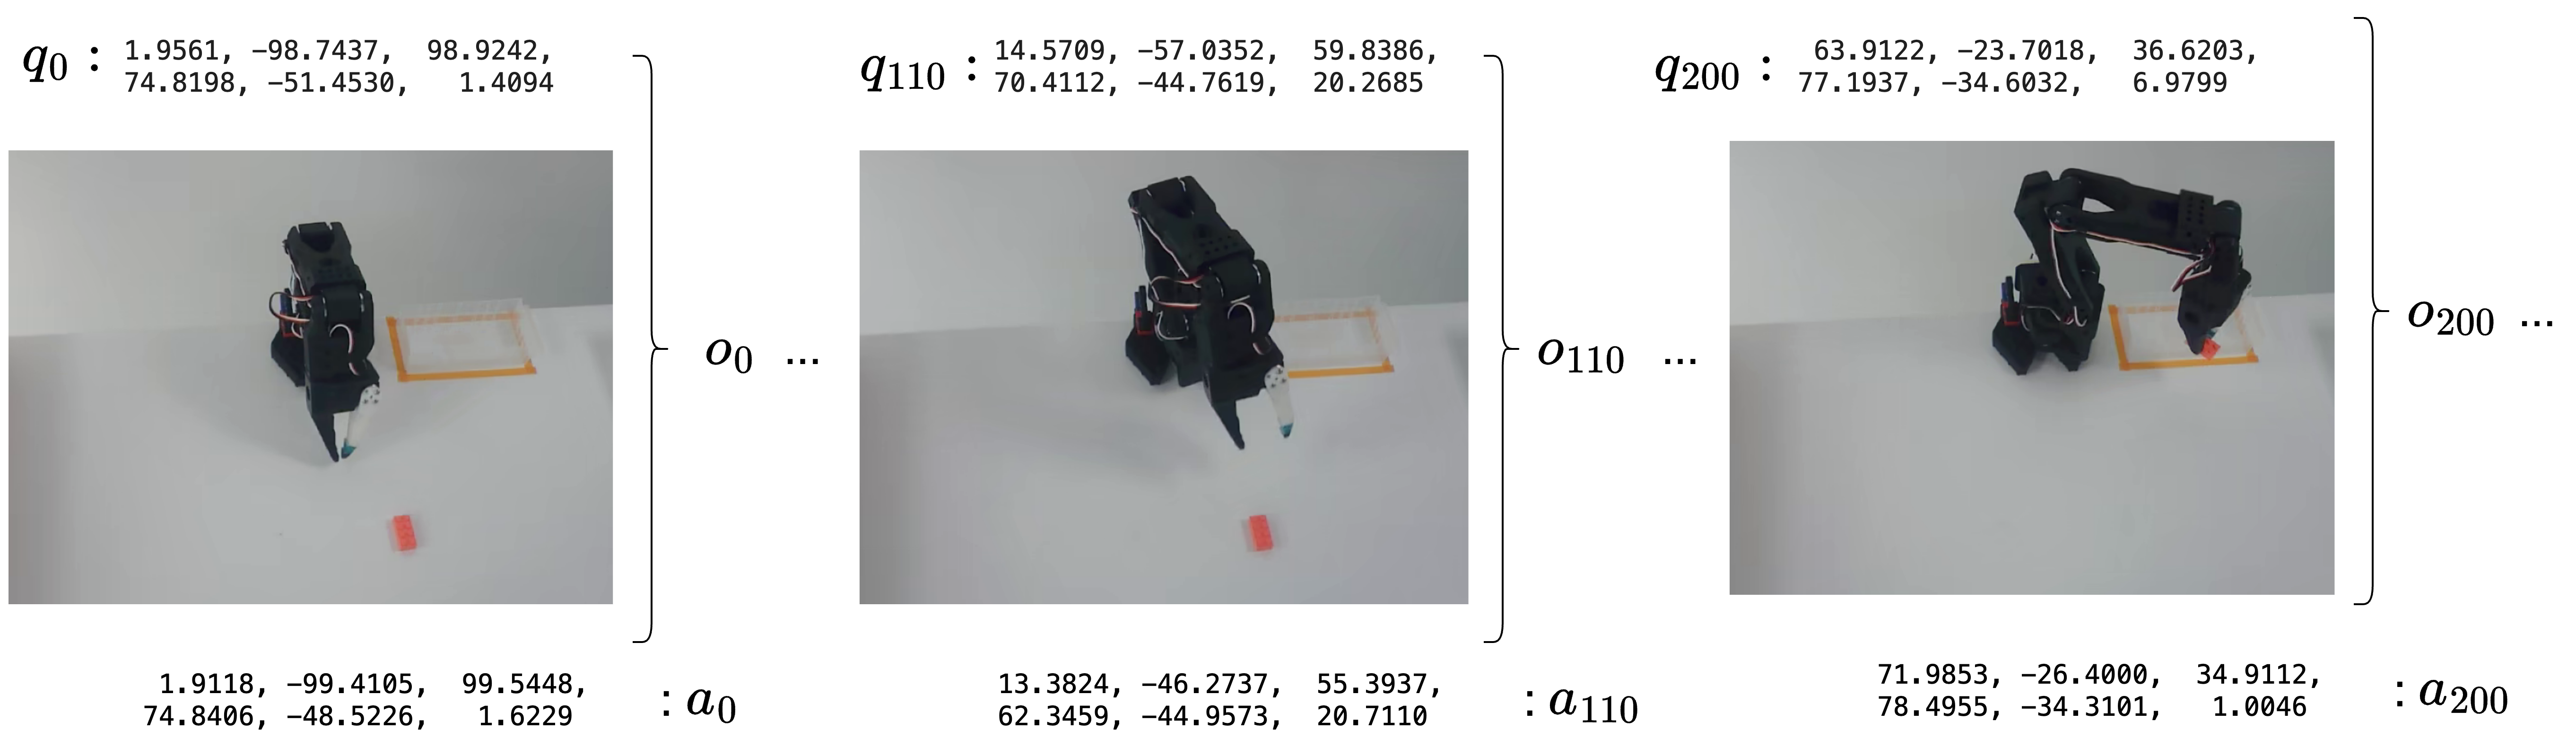
\includegraphics[width=0.9\textwidth]{figures/ch4/ch4-observation-action-mapping.png}
    \caption{Sample observations and action pairs over the course of a given trajectory recorded in \url{lerobot/svla_so101_pickplace}. Observations, comprising of both proprioperceptive and visual information, are recorded alongside the configuration of a second, leader robot controlled by a human expert, providing complete information for regressing actions given observations.}
    \label{fig:ch4-observation-action-mapping}
\end{figure}

Behavioral Cloning (BC)~\citep{pomerleauALVINNAutonomousLand1988} aims at producing synthetic behaviors by learning the mapping from observations to actions, and in its most natural formulation can be effectively tackled as a \emph{supevised} learning problem, consisting of learning the (deterministic) mapping \(f: \obsspace \mapsto \actionspace, \ a_t = f(o_t) \) by solving
\begin{equation}\label{eq:loss-minimization-SL}
    \min_{f} \mathbb{E}_{(o_t, a_t) \sim p(\bullet)} \mathcal L(a_t, f(o_t)),
\end{equation}
given an arbitrary risk function \( \mathcal L:  \mathcal A \times \mathcal A \mapsto \mathbb{R}, \ \mathcal L (a, a^\prime) \).

Typically, the expert's joint observation-action distribution \( p: \obsspace \times \actionspace \mapsto [0,1] \) is assumed to be unknown, in keeping with a classic Supervised Learning (SL) framework\footnote{Throughout, we will adopt the terminology and notation for SL used in~\citet{shalev-shwartzUnderstandingMachineLearning2014}}.
However, differently from standard SL assumptions, the samples collected in \( \mathcal D \)---realizations of the underlying \( p \)---are \emph{not} i.i.d., as expert demonstrations are collected \emph{sequentially} in the form of trajectories.
In practice, this aspect can be partially mitigated by considering pairs in a non-sequential order---\emph{shuffling} the samples in \(\mathcal D \)---so that the expected risk under \( p \) can be approximated using MC estimates, although these estimates may in general be less accurate.
Another strategy to mitigate the impact of regressing over non-i.i.d. samples relies on the possibility of interleaving BC and data collection~\citep[DAgger]{rossReductionImitationLearning2011}, aggregating multiple datasets iteratively.
However, because we only consider the case where a single offline dataset \( \mathcal D \) of trajectories is available and no more data can be collected, DAgger falls out of our scope.

Despite the inherent challenges of learning from non-i.i.d. data, the BC formulation presents several operational advantages in robotics.
First, training happens offline and naturally accomodates for expert, demonstration data, hereby severily limiting exploration risks by preventing the robot from performing dangerous actions altogether, by anchoring action in imitation.
Second, reward design is entirely unnecessary in BC, as demonstrations already reflect human intent.
The absence of rewards also prevents the risk of misalignment and specification gaming (\emph{reward hacking}), otherwise inherent in purely reward-based RL~\citep{heessEmergenceLocomotionBehaviours2017}.
Third, because expert trajectories encode terminal conditions, success detection and resets are implicit in the dataset.
Finally, empirical evidence suggests the performance of BC scales naturally with growing corpora of demonstrations collected across tasks, embodiments, and environments.
Nonetheless, BC can, in principle, only reproduce behaviors that are at best as good as those of the demonstrator, and therefore offers no remedy for the suboptimal decisions that humans may enact.
This limitation is particularly problematic in sequential decision-making tasks where expert demonstrations are scarce--—either because data collection is costly or because human performance is inherently suboptimal. 
Yet, many robotics applications still benefit from relatively inexpensive pipelines for collecting high-quality human-generated trajectories, justifying the use of BC in such settings.

\begin{figure}
    \centering
    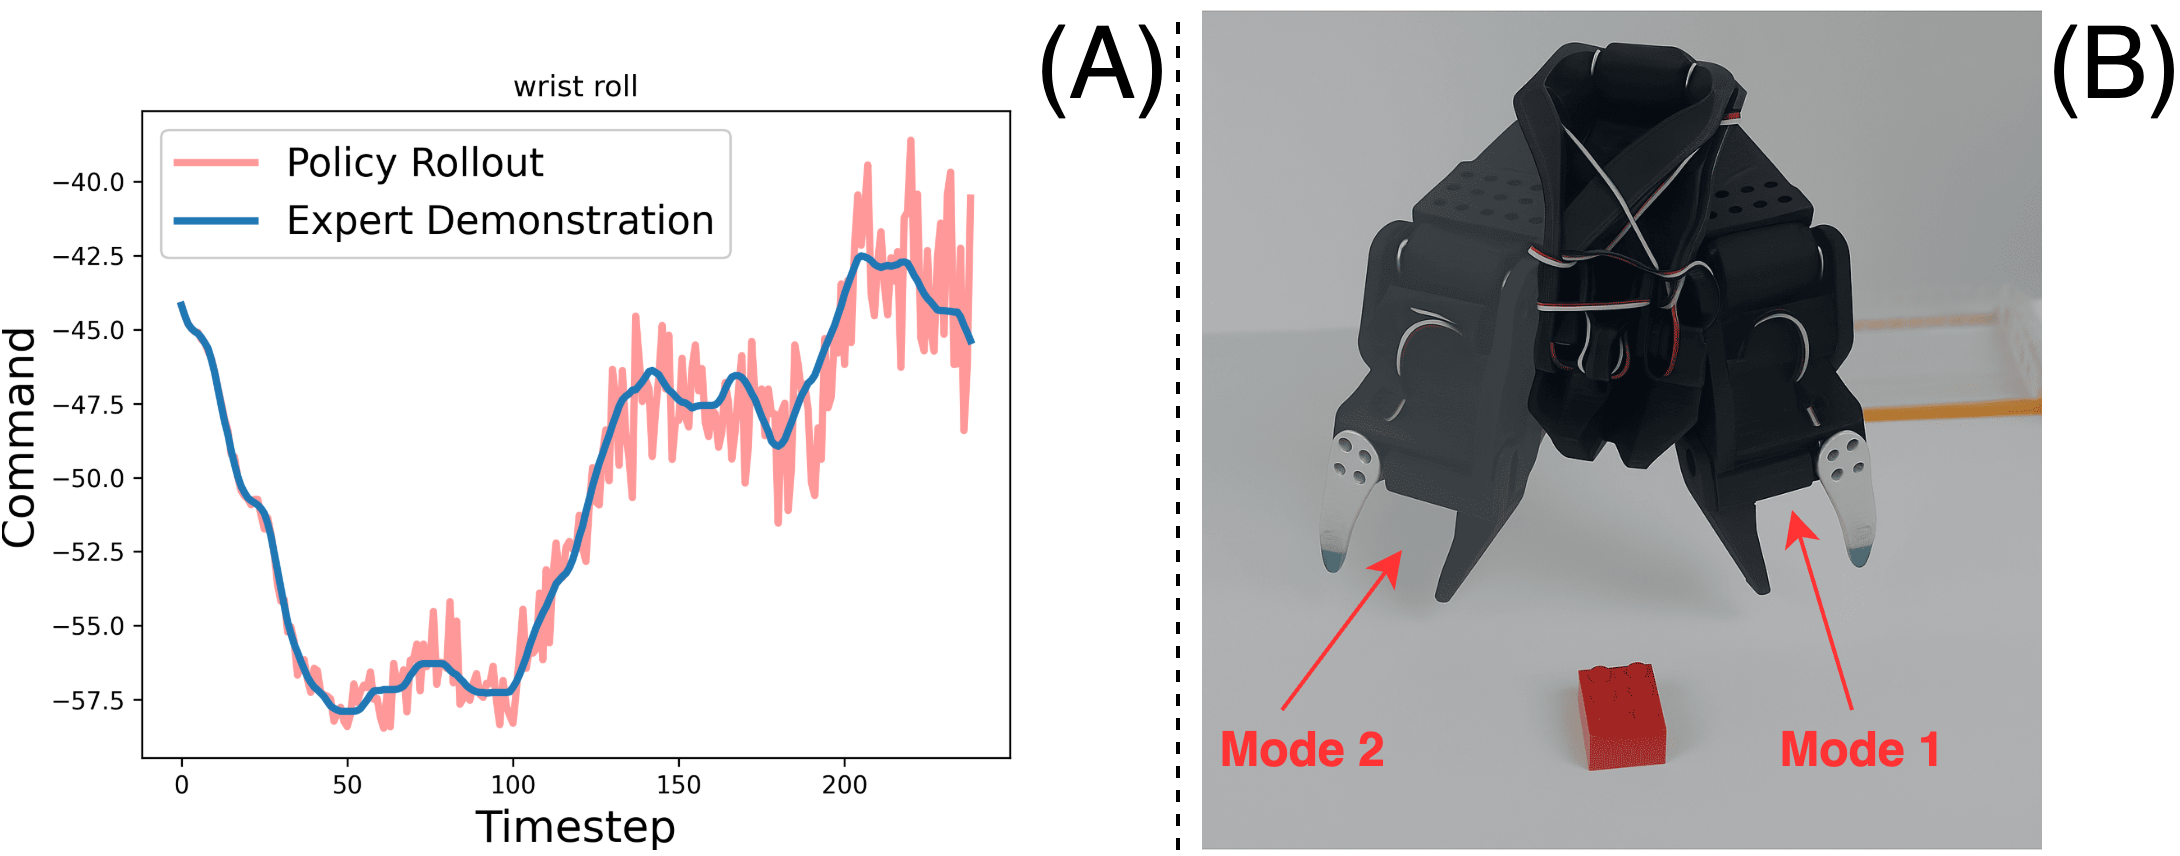
\includegraphics[width=0.8\textwidth]{figures/ch4/ch4-issues-with-bc.png}
    \caption{Point-wise policies suffer from limitations due to (A) covariate shifts and (B) poor approximation of multimodal demonstrations. (A) Small errors may drive the policy out of distribution, incuring in a vicious circle ultimately resulting in failure. (B) Both modes of reaching for a target object in the scene---either left or right-first---are equally as good and thus equally as likely to be present in a dataset of human demonstrations, ultimately resulting in multimodal demonstrations.}
    \label{fig:ch4-issues-with-bc}
\end{figure}

While conceptually elegant, \emph{point-estimate policies} \( f : \obsspace \mapsto \actionspace \) learned by solving eq.~\ref{eq:loss-minimization-SL} have been observed to suffer from (1) compounding errors~\citep{rossReductionImitationLearning2011} and (2) poor fit to multimodal distributions~\citep{florenceImplicitBehavioralCloning2022, keGraspingChopsticksCombating2020}.
Figure~\ref{fig:ch4-issues-with-bc} illustrates these two key issues related to learning \emph{explicit policies}~\citep{florenceImplicitBehavioralCloning2022}.
Besides sequentiality in \( \mathcal D \), compounding errors due to \emph{covariate shift} may also prove catastrophic, as even small \( \epsilon \)-prediction errors \( 0 < \Vert \mu(o_t) - a_t \Vert \leq \epsilon \) can quickly drive the policy into out-of-distribution states, incuring in less confident generations and thus compounding errors (Figure~\ref{fig:ch4-issues-with-bc}, left).
Moreover, point-estimate policies typically fail to learn \emph{multimodal} targets, which are very common in human demonstrations solving real-world robotics problems, as multiple trajectories can be equally as good towards the accomplishment of a goal (e.g., symmetric grasps, Figure~\ref{fig:ch4-issues-with-bc}, right).
In particular, unimodal regressors tend to average across modes, yielding indecisive or even unsafe commands~\citep{florenceImplicitBehavioralCloning2022}.
To address poor multimodal fitting,~\citet{florenceImplicitBehavioralCloning2022} propose learning the \emph{generative model} \( p(o, a) \) underlying the samples in \( \mathcal D \), rather than explicitly learning a prediction function \( f: a = f(o) \).

\subsection{A (Concise) Introduction to Generative Models}
% Generative Modeling
Generative Models (GMs) aim to learn the stochastic process underlying the very generation of the data collected, and typically do so by fitting a probability distribution that approximates the unknown \emph{data distribution}, \( p \).
In keeping with the GM literature, \( p(x) \leftarrow \mathbb P(x), x \sim p \).
In the case of BC, the unknown data distribution \( p \) may represent the expert's joint distribution over \( (o, a) \)-pairs.
Thus, given a finite set of \( N \) pairs \(\mathcal D = \{ (o,a)_i \}_{i=0}^N\) available as an imitation learning target (and thus assumed to be i.i.d.), GMs seek to learn a \emph{parametric} distribution \( p_\theta(o,a) \) such that (1) new samples \( (o,a) \sim p_\theta(\bullet) \) resemble those stored in \( \mathcal D \), and (2) high likelihood is assigned to the \emph{observed} regions of the \emph{unobservable} \( p \).
Likelihood-based learning provides a principled training objective to achieve both goals, and it is thus extensively used in GMs~\citep{prince2023understanding}.

% VAEs
\subsubsection{Variational Auto-Encoders}

\begin{figure}
    \centering
    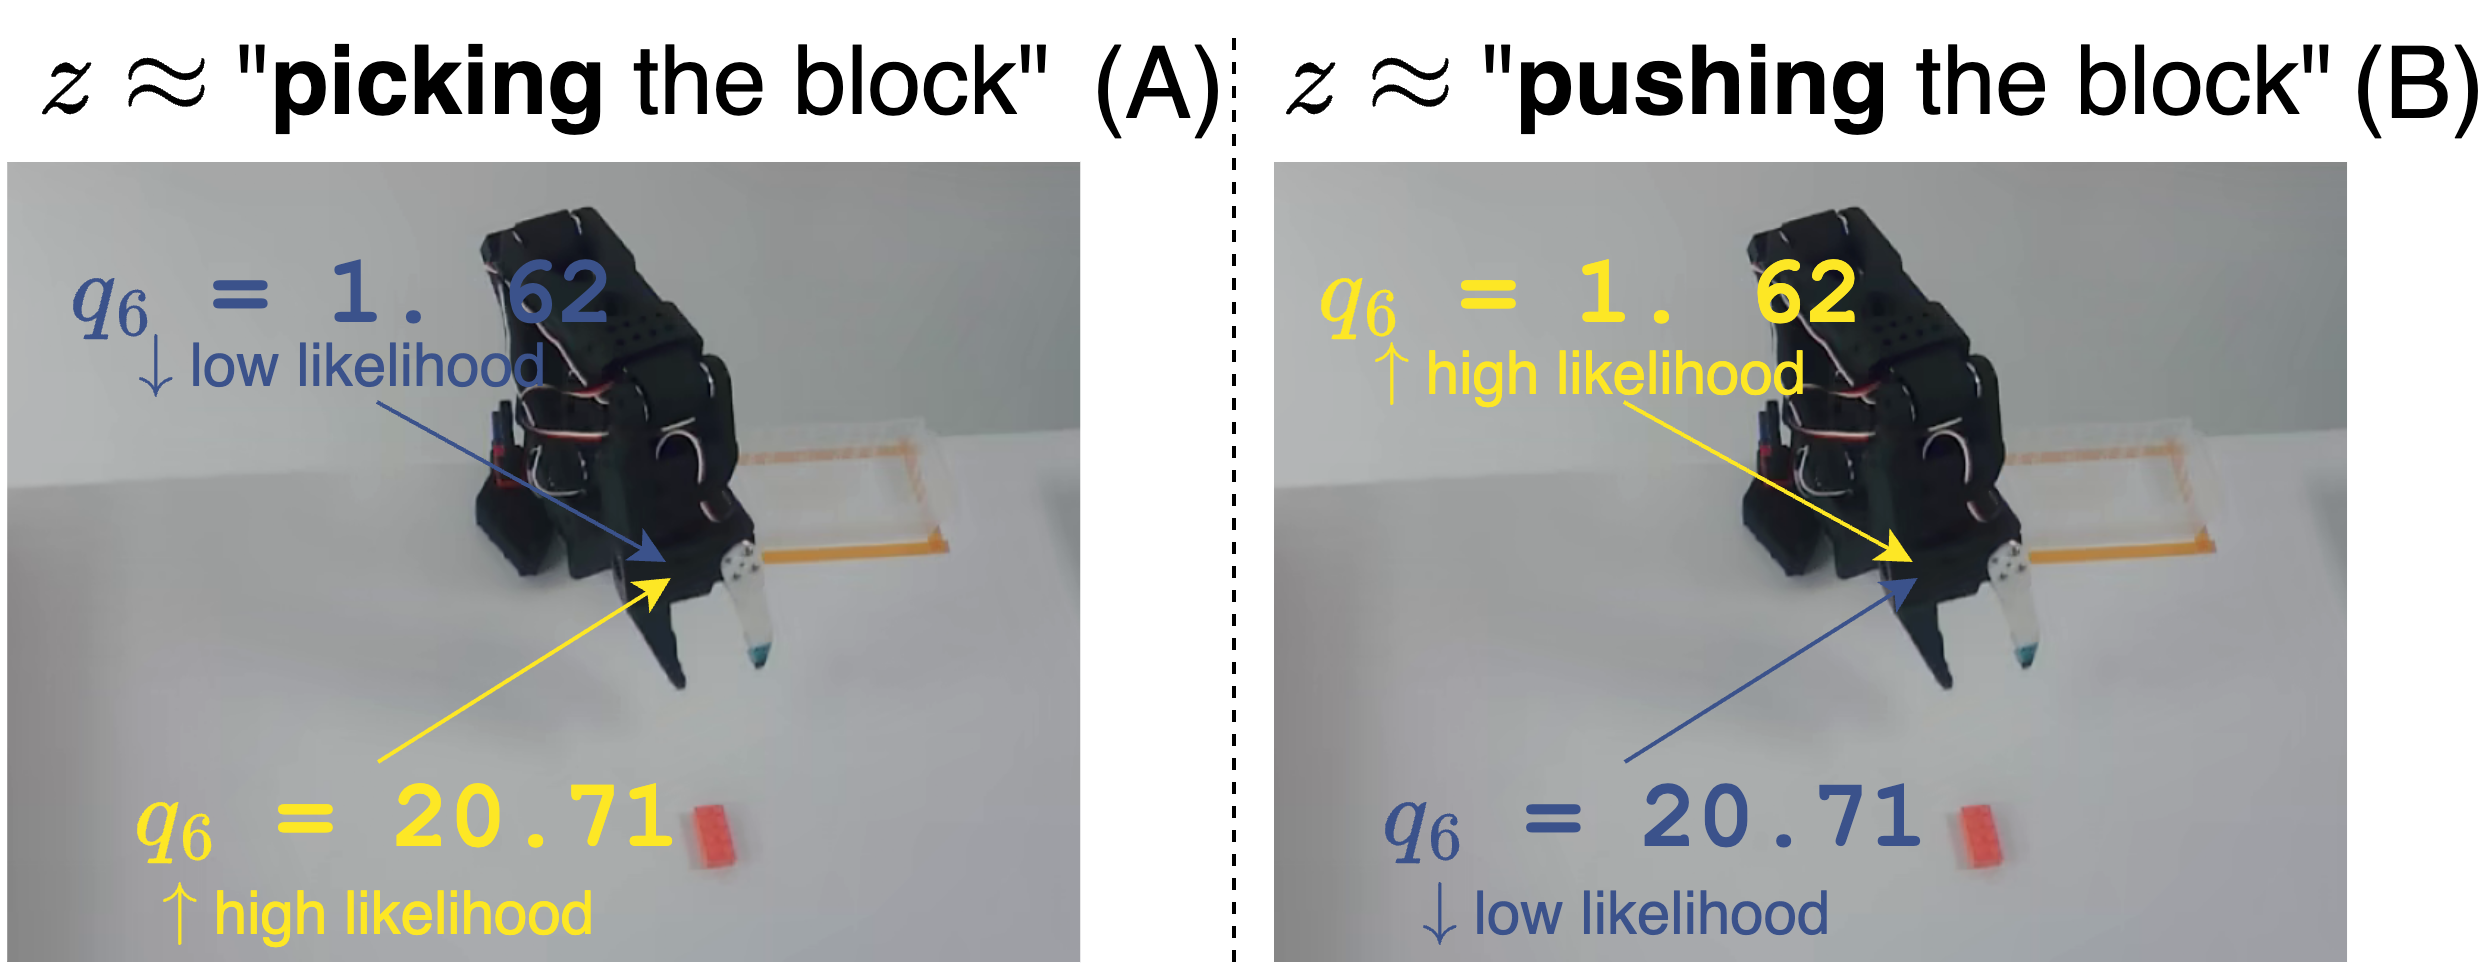
\includegraphics[width=0.8\textwidth]{figures/ch4/ch4-task-effect-on-pairs.png}
    \caption{Intuitively, latent variable in a single latent model may contain information regarding the task being performed, which directly results in the likelihood of the same observation-action pair being different for two different tasks. When (A) picking a block the likelihood of a wide gripper's opening should be higher than narrower one, while it should be the opposite when (B) pushing the block.}
    \label{fig:ch4-task-effect-on-pairs}
\end{figure}

A common inductive bias used in GM posits samples \( (o,a) \) are influenced from an unobservable latent variable \( z \in Z \), resulting in:
\begin{equation}\label{eq:BC-latent-variable}
    p (o,a) = \int_{\supp{Z}} p(o,a \vert z) p(z)
\end{equation}
Intuitively, in the case of observation-action pairs \( (o, a) \) for a robotics application, \( z \) could be interpreted as some high level representation of the underlying task being performed by the human demonstrator.
In such case, treating \( p(o,a) \) as a marginalization over \( \supp{Z} \) of the complete joint distribution \( p(o,a,z) \) natively captures the effect different tasks have on the likelihood of observation-action pairs.
Figure~\ref{fig:ch4-task-effect-on-pairs} graphically illustrates this concept in the case of a (A) picking and (B) pushing task, for which, nearing the target object, the likelihood of actions resulting in opening the gripper---the higher \( q_6 \), the wider the gripper's opening---should intuitively be (A) high or (B) low, depending on the task performed.
While the latent space \( Z \) typically has a much richer structure than the set of all actual tasks performed, eq.~\ref{eq:BC-latent-variable} still provides a solid framework to learn joint distribution conditioned on unobservable yet relevant factors.
Figure~\ref{fig:ch4-latent-variable-model} represents this latent-variable framework in the context of a robotics application: the true, \( z \)-conditioned generative process assigns \emph{likelihood} \( p((o,a) \vert z) \) to the single \( (o,a) \)-pair.
Using Bayes' theorem, one can reconstruct the \emph{posterior} distribution on \( \supp{Z} \), \( q_\theta(z \vert o,a) \) from the likelihood \( p_\theta(o,a \vert z) \), \emph{prior} \( p_\theta(z) \) and \emph{evidence} \( p_\theta(o,a) \).
VAEs approximate the latent variable model presented in eq.~\ref{eq:BC-latent-variable} using an \emph{approximate posterior} \(q_\phi(z \vert o,a) \) while regressing parameters for a parametric likelihood, \( p_\theta(o,a \vert z) \) (Figure~\ref{fig:ch4-latent-variable-model}).

\begin{figure}
    \centering
    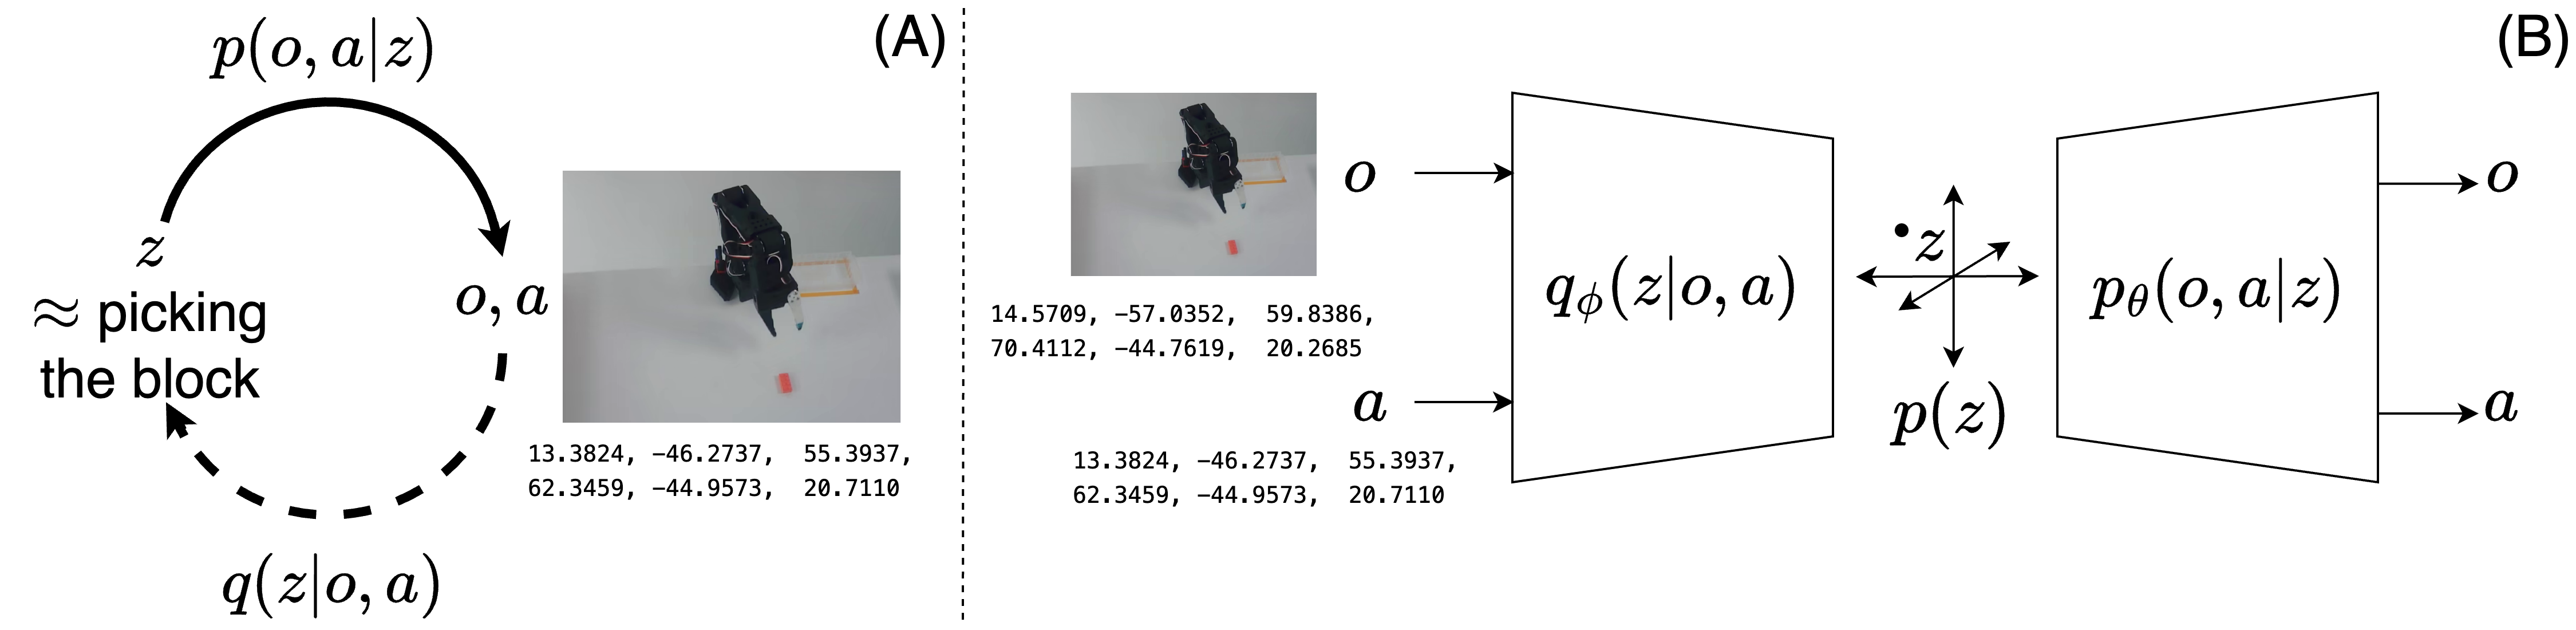
\includegraphics[width=0.9\textwidth]{figures/ch4/ch4-latent-variable-model.png}
    \caption{(A) The latent variable model in a robotics application regulates influence between observed (\(o,a) \) variables and an unobservable latent variable. (B) VAEs approximate exact latent variable models by means of variational inference. }
    \label{fig:ch4-latent-variable-model}
\end{figure}

Given a dataset \( \mathcal D \) consisting of \( N \) i.i.d. observation-action pairs, the log-likelihood of all datapoints under \( \theta \) (in Bayesian terms, the \emph{evidence} \( p_\theta(\mathcal D)\)) can be written as:
\begin{align}
    \log p_\theta(\mathcal D) &= \log \sum_{i=0}^N p_\theta ((o,a)_i) \label{eq:evidence-definition-1}\\
                              &= \log \sum_{i=0}^N \int_{\supp{Z}} p_\theta((o,a)_i \vert z) p(z) \label{eq:evidence-definition-2}\\
                              &= \log \sum_{i=0}^N \int_{\supp{Z}} \frac{q_\theta(z \vert (o,a)_i)}{q_\theta(z \vert (o,a)_i)} \cdot p_\theta((o,a)_i \vert z) p(z) \label{eq:evidence-definition-3}\\
                              &= \log \sum_{i=0}^N \mathbb E_{z \sim q_\theta(\bullet \vert (o,a)_i)} \left[ \frac{p(z)}{q_\theta(z \vert (o,a)_i)} \cdot p_\theta((o,a)_i \vert z) \right], \label{eq:evidence-definition}
\end{align}
where we used eq.~\ref{eq:BC-latent-variable} in eq.~\ref{eq:evidence-definition-1}, multiplied by \(1 = \frac{q_\theta(z \vert (o,a)_i)}{q_\theta(z \vert (o,a)_i)} \) in eq.~\ref{eq:evidence-definition-2}, and used the definition of expected value in eq.~\ref{eq:evidence-definition}.

In the special case where one assumes distributions to be tractable, \( p_\theta (\mathcal D) \) is typically tractable too, and \(\max_\theta \log p_\theta(\mathcal D) \) provides a natural target for (point-wise) infering the unknown parameters \( \theta \) of the generative model.
Unfortunately, eq.~\ref{eq:evidence-definition} is rarely tractable when the distribution \( p \) is modeled with approximators such as neural networks, especially for high-dimensional, unstructured data.

In their seminal work on Variational Auto-Encoders (VAEs),~\citet{kingma2013auto} present two major contributions to learn complex latent-variable GMs from unstructured data, proposing (1) a tractable, variational lower-bound to eq.~\ref{eq:evidence-definition} as an optimization target to jointly learn likelihood and posterior and (2) using high-capacity function approximators to model the likelihood \(p_\theta(o,a\vert z)\) and (approximate) posterior distribution \( q_\phi(z \vert o,a) \approx q_\theta(z \vert o,a) \).

In particular, the lower bound on eq.~\ref{eq:evidence-definition} (Evidence LOwer Bound, \emph{ELBO}) can be derived from eq.~\ref{eq:evidence-definition} applying Jensen's inequality---\(\log \mathbb{E}[\bullet] \geq \mathbb{E} [\log (\bullet)] \)---yielding:
\begin{align}
    \log p_\theta(\mathcal D) &\geq \sum_{i=0}^{N} \left(
            \mathbb{E}_{z \sim q_\theta(\bullet \vert (o,a)_i)} \big[ \log p_\theta((o,a)_i \vert z) \big]
            + \mathbb{E}_{z \sim q_\theta(\bullet \vert (o,a)_i)} \left[ \log \left( \frac{p(z)}{q_\theta(z \vert (o,a)_i)} \right) \right]
        \right) \\
        &= \sum_{i=0}^{N} \left(
            \mathbb{E}_{z \sim q_\theta(\bullet \vert (o,a)_i)} \big[ \log p_\theta((o,a)_i \vert z) \big]
        - \DKL \big[ q_\theta(z \vert (o,a)_i) \Vert p(z) \big]
        \right) \label{eq:ELBO-intractable}
\end{align}

The true, generally intractable, posterior \( q_\theta (z \vert o,a) \) prevents computing both the expectation and KL divergence terms in eq.~\ref{eq:ELBO-intractable}, and therefore~\citet{kingma2013auto} propose deriving the ELBO using an \emph{approximate} posterior \( q_\phi(z \vert o,a) \), resulting in the final, tractable, ELBO objective,
\begin{align}
\text{ELBO}_{\mathcal D}(\theta, \phi) = \sum_{i=0}^{N} \left(
            \mathbb{E}_{z \sim q_\phi(\bullet \vert (o,a)_i)} \big[ \log p_\theta((o,a)_i \vert z) \big]
        - \DKL \big[ q_\phi(z \vert (o,a)_i) \Vert p(z) \big]
        \right)
        \label{eq:ELBO}
\end{align}
From Jensen's inequality, maximizing ELBO results in maximizing the log-likelihood of the data too, thus providing a natural, tractable optimization target.
Indeed, expectations can be estimated using MC estimates from the learned distributions in eq.~\ref{eq:ELBO}, while the KL-divergence term can typically be computed in closed-form (1) modeling  \(q_\phi \) as a Gaussian \(q_\phi(z \vert o,a) = \mathcal N\big(\mu_\phi(o,a), \Sigma_\phi(o,a) \big) \) with learned mean vector \( \mu_\phi(o,a) \) and learned variance-covariance matrix \( \Sigma_\phi(o,a) \) and (2) imposing a standard Gaussian prior on the latent space, \( p(z) = \mathcal N(\mathbf{0}, \mathbf{I}) \).

An intuitive explanation of the learning dynamics of VAEs can be given considering the equivalent case of \emph{minimizing the negative ELBO}, which admits the particularly interpretable factorization (considering, without loss of generality, only one \( (o,a) \sim \mathcal D \)):
\begin{align}
\min_{\theta, \phi} - \text{ELBO}_{\mathcal (o,a) \sim \mathcal D}(\theta, \phi) &= \min_{\theta, \phi}\mathbf{L^{\text{rec}}}(\theta) + \mathbf{L^{\text{reg}}}(\phi), \label{eq:VAE-min-neg-ELBO}\\
\mathbf{L^{\text{rec}}}(\theta) &= \mathbb{E}_{z \sim q_\phi(\bullet \vert o,a}) \big[ \log p_\theta(o,a \vert z) \big] \label{eq:VAE-Lrec} \\
\mathbf{L^{\text{reg}}}(\phi) &= \DKL \big[ q_\phi(z \vert o,a) \Vert p(z) \big]. \label{eq:VAE-Lreg}
\end{align}

For any given \((o,a) \) pair, the expected value term in eq.~\ref{eq:VAE-Lrec} is typically computed via MC estimates, resulting in
\[ 
-\mathbb{E}_{z \sim q_\phi(\bullet \vert o,a)} \big[ \log p_\theta(o,a \vert z) \big] = \mathbf{L^{\text{rec}}} \approx - \frac{1}{n} \sum_{i=0}^n \log p_\theta(o,a \vert z_i).
\]
Assuming \( p_\theta(o,a \vert z) \) to be parametrized with an isotropic Gaussian distribution with mean \(\mu_\theta (z) \in \mathbb R^d \) and variance \( \sigma^2 \), the log-likelihood thus simplifies to:
\[
\log p(o,a \vert z_i) = -\frac{1}{2\sigma^{2}} \big \Vert (o,a)-\mu_\theta(z_i) \big\Vert_2^2 -\frac{d}{2}\log(2\pi \sigma^{2}) \implies \mathbf{L^\text{rec}} \approx \frac {1}{n} \sum_{i=0}^n \big\Vert (o,a) - \mu_\theta(z_i) \big \Vert^2_2
\]
In practice, it is common to approximate the learned likelihood \( p_\theta(o,a \vert z) \) with a parametric distribution (e.g., Gaussian) whose parameters are given by a learned coefficient vector derived from \( \mu_\theta(z), \ z \sim p(\bullet) \). 
Under this formulation, learning a VAE amounts to (1) \emph{reconstructing} the examples in \( \mathcal{D} \) by minimizing (1) the reconstruction loss \( \mathbf{L^{\text{rec}}}\)---a standard \emph{supervised learning} objective for regression---while (2) \emph{regularizing} the latent representation by minimizing \( \mathbf{L^{\text{reg}}} \). 
The latter enforces information compression, since with the common prior choice \( p(z) = \mathcal{N}(\mathbf{0}, \mathbf{I})\) in eq.~\ref{eq:VAE-Lreg}, the regularizer constrains the posterior and thereby limits the expressivity of \( q_\phi(z \vert o,a) \).

% Diffusion
\subsubsection{Diffusion Models}
VAEs approximate probability distributions via a \emph{single} latent variable model, assuming the underlying unknown distribution can be factored according to eq.~\ref{eq:BC-latent-variable}, and solve the variational-inference problem of jointly learning the likelihood \( p_\theta \) and (approximate) posterior \( q_\phi \) for such model.
In that, the unknown data distribution \( p(o,a) \) is effectively approximated via \( \int_Z p(z) p_\theta(o,a \vert z) \), and the underlying generative process reproduced by (1) sampling a latent variable and (2) learning to decode it into a high-likelihood sample under the (unknown) \( p(o,a) \).
Diffusion Models (DMs)~\citep{hoDenoisingDiffusionProbabilistic2020} are another class of GMs which treat the similar problem of approximating an underlying unknown data distribution---\emph{variational inference}---by \emph{partially} extending VAEs to the case where \emph{multiple} latent variables influence each other and the generative process underlying \(o,a\) itself.
In particular, DMs posit the generative process can be decomposed to a series of piece-wise (Markovian) interactions between (latent) variables (Figure~\ref{fig:ch4-many-latents}), resulting in
\begin{align}
    p(\underbrace{o,a}_{= z_0}) &= \int_{\supp{Z_0}} \int_{\supp{Z_1}} \hdots \int_{\supp{Z_T}} p(z_0, z_1, \dots z_T) \label{eq:BC-multi-latent-model-1} \\ 
    p(z_0, z_1, \dots z_T) &= p(z_T) \prod_{t=1}^{T} p(z_{t-1} \vert z_t), \label{eq:BC-multi-latent-model-2}
\end{align}
where we explicitly showed the marginalization over the multiple latents in eq.~\ref{eq:BC-multi-latent-model-1}, and used the law of conditional probability and Markov property in eq.~\ref{eq:BC-multi-latent-model-2}.
Also, for ease of notation, we will refer to observation-action pairs \( o,a \) as \( z_0 \).

\begin{figure}
    \centering
    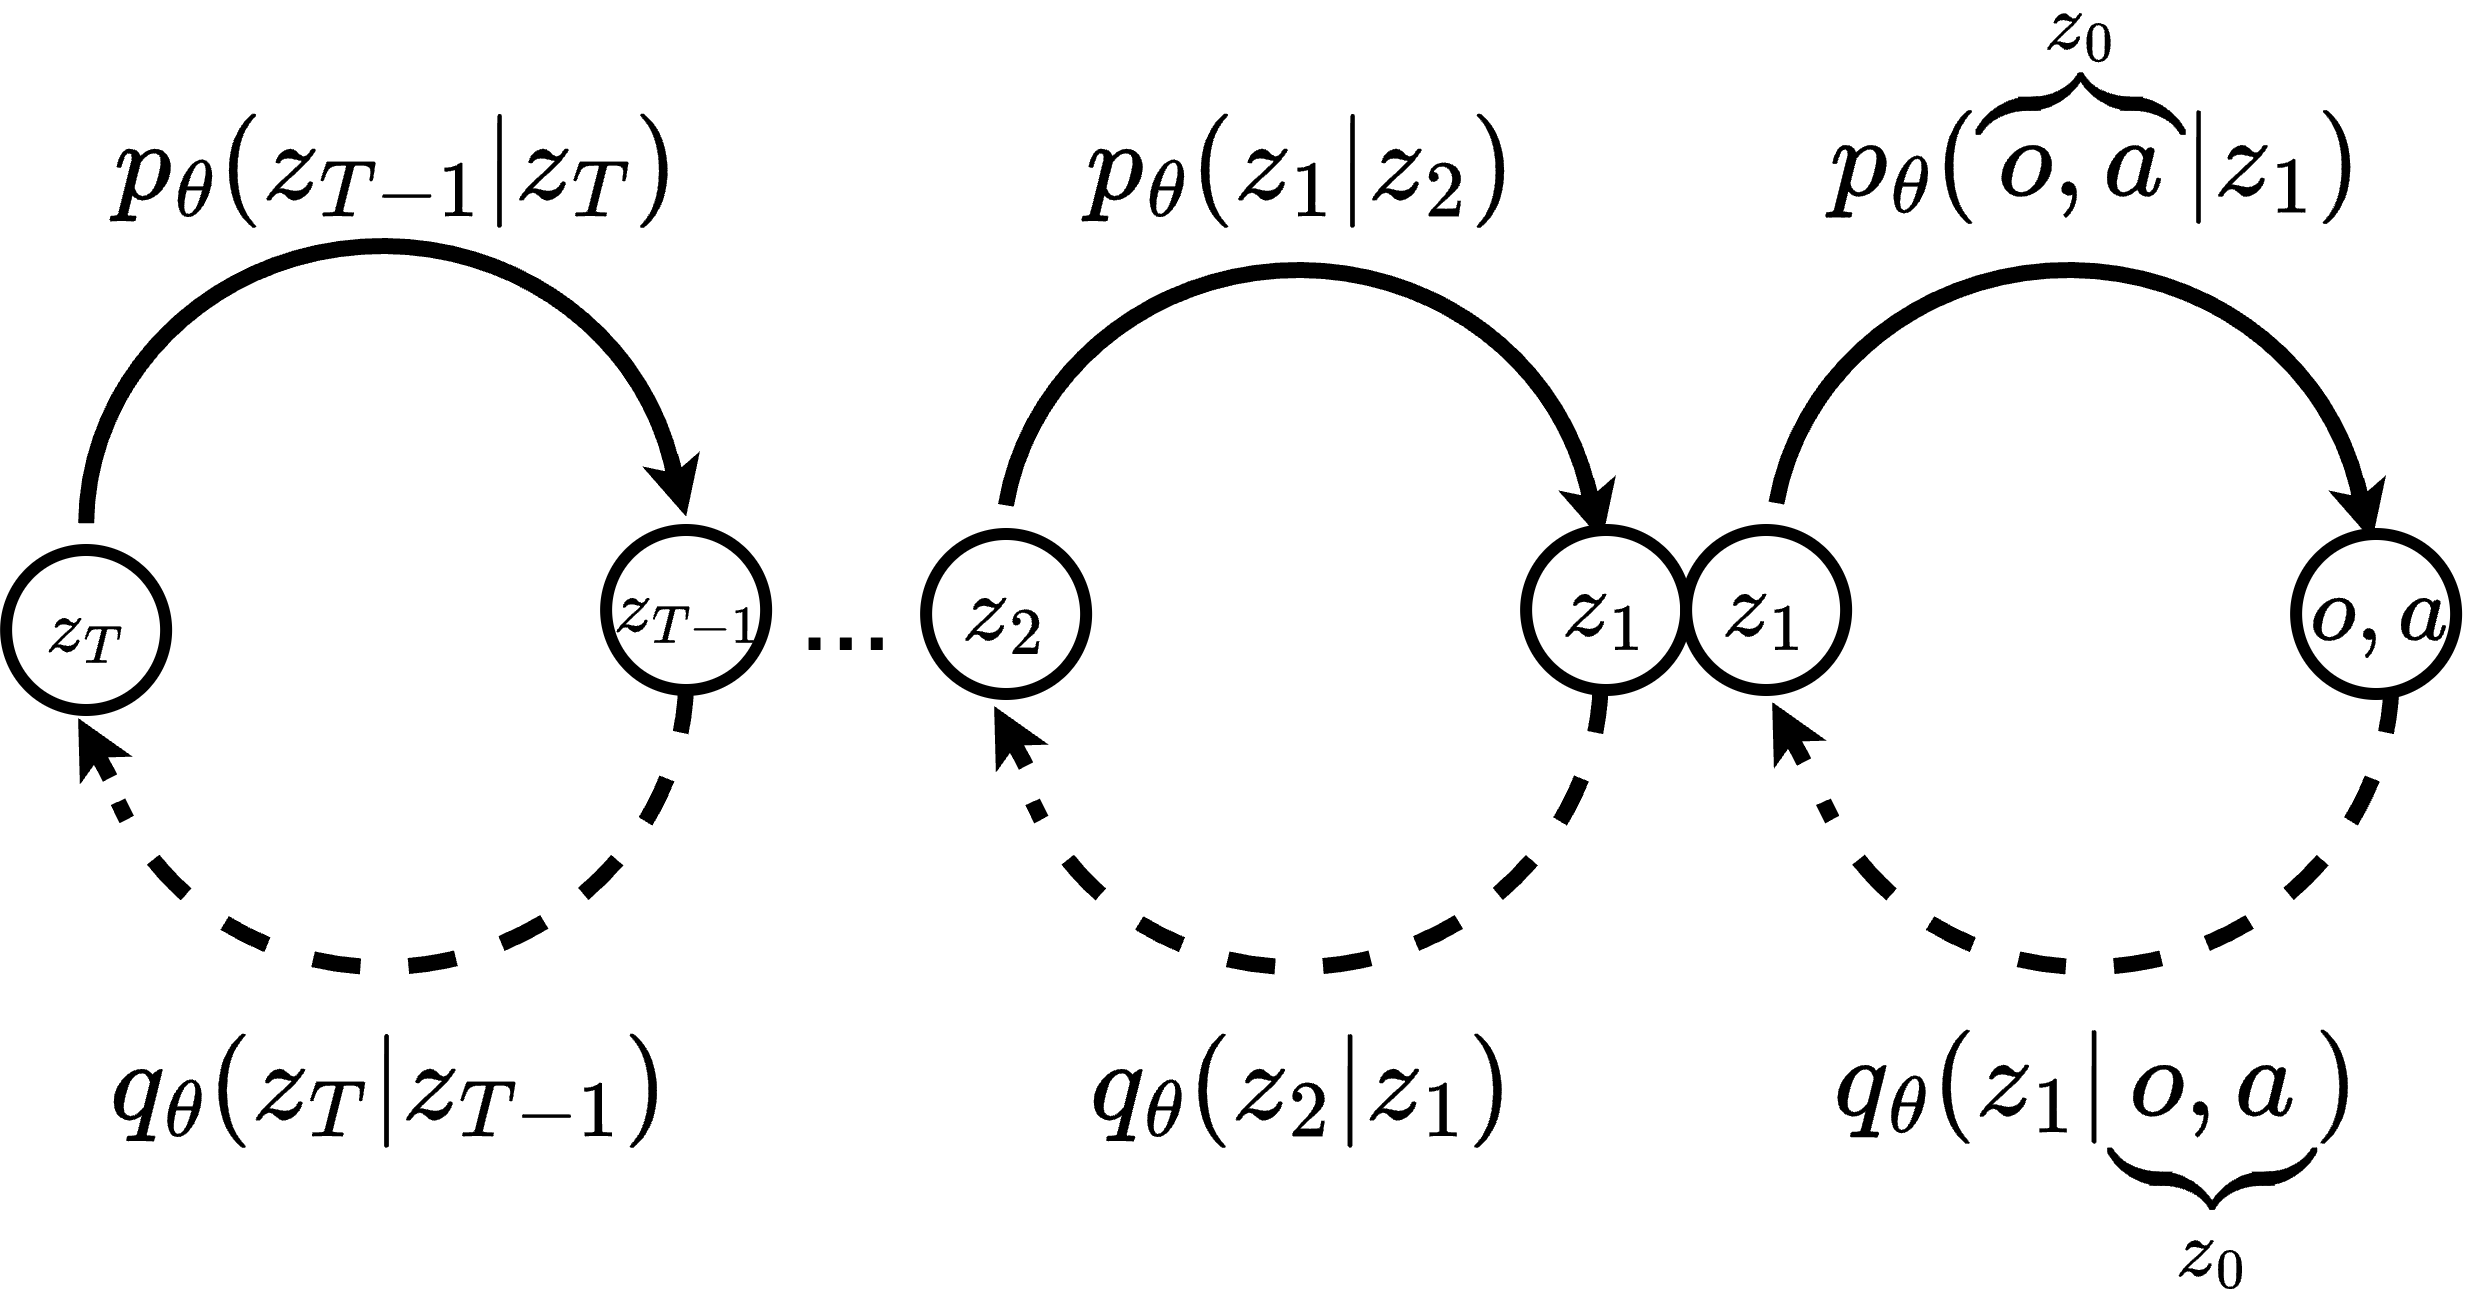
\includegraphics[width=0.5\textwidth]{figures/ch4/ch4-many-latents.png}
    \caption{HMLV models posit the data generation process is influenced by a stack of Markov-dependent latent variables, with samples from the posterior distribution being progressively higher up in the hierarchy.}
    \label{fig:ch4-many-latents}
\end{figure}

Similar to VAEs, it is generally not possible to assign an \emph{exact} interpretation to the latent variables. 
Nevertheless, a reasonable application-driven intuition is that Hierarchical Markov Latent Variable (HMLV) models, by capturing hierarchical and decoupled interactions among latent variables, can reflect the different resolutions at which conditioning factors intervene. 
For example, in a robotics setting, one might naturally distinguish between high-level trajectory planning (higher up in the hierarchy, \(t \to T\)) and fine-grained motion adjustments (closer to empirical observations, \(t \to 0\)).
In that, HMLV models thus provide a framework to perform variational inference via multiple, sequential sampling steps from different higher level distributions instead of approximating the generative process with a single-latent variable model.
DMs are a particular instantiation of HMLV models for which the posterior is fixed to \( q( z_t \vert z_{t-1}) = \mathcal N(z_t \sqrt{1-\beta_t}, \beta_t \mathbf{I}) \), for a given \( \beta_t \in \mathbb R^+ \). 
In practice, \( \beta_t \) is used to iteratively reduce the signal-to-noise ratio along the latents' hierarchy, similarily to how a diffusion process influences the information of a physical system.

Just like VAEs, DMs attemp to learn to reproduce an underlying data distribution \( p (o,a) \) given a collection of i.i.d. samples approximating the model posited to have generated the data in the first place (eq.~\ref{eq:BC-multi-latent-model-1}).
Similarily to VAEs, DMs approximate the process of sampling from the unknown \( p(o,a) \) by (1) sampling from an easy-to-sample distribution (e.g., Gaussian) and (2) learning to reconstruct high-likelihood samples under the unknown distribution.
However, in stark contrast with VAEs, the easy-to-sample distribution contains \emph{no mutual information} regarding the data distribution \( p(o,a) \).
Crucially, as no information from the sample \( (o,a) \) (denoted as \( z_0 \equiv (o,a) \) for simplicity of notation) is assumed to be propagated throughout the chain of latents, the posterior \( q(z_t \vert z_{t-1})\) assumes a relatively amicable structure in DMs, reducing complexity.
The \emph{true} likelihood \( p(z_{t-1} \vert z_t) \) is instead typically approximated using the parametrization \(  p_\theta (z_{t-1} \vert z_t) \).
In that, the information contained in the unknwon data distribution is \emph{reconstructed} via a process in which samples from a fixed distribution are iteratively turned into (ideally) high-likelihood samples under \( p(o,a) \)---a process referred to as \emph{denoising}.

Under such model, we can express the log-likelihood of an arbitrary sample \( z_0 \) as:
\begin{align}
    \log p_\theta (z_0) &= \log \int_{\supp{Z_1} \times \supp{Z_2} \times \dots \times \supp{Z_T}} p_\theta(\underbrace{z_0, z_1, z_2, \dots z_T}_{z_{0:T}}) \\
    &= \log \int_{\supp{Z_{1:T}}} \frac{p_\theta(z_{0:T}) \cdot q(z_{1:T} \vert z_0)}{q(z_{1:T} \vert z_0)} \label{eq:diffusion-1} \\
    &= \log \mathbb{E}_{z_{1:T} \sim q(\bullet \vert z_0)} \bigg[ \frac{p_\theta(z_{0:T})}{q(z_{1:T} \vert z_0)} \bigg] \\
    &\geq \mathbb{E}_{z_{1:T} \sim q(\bullet \vert z_0)} \bigg[ \log \frac{p_\theta(z_{0:T})}{q(z_{1:T} \vert z_0)} \bigg] \label{eq:diffusion-jensen} \\
    &= \mathbb{E}_{z_{1:T} \sim q(\bullet \vert z_0)} \bigg[ \log \frac{p(z_T) \prod_{t=1}^{T} p_\theta (z_{t-1} \vert z_t)}{\prod_{t=1}^T q(z_t \vert z_{t-1})} \bigg] \label{eq:diffusion-2} \\
    &= \mathbb{E}_{z_{1:T} \sim q(\bullet \vert z_0)} \bigg[ \log \frac{p(z_T) \cdot p_\theta (z_0 \vert z_1) \prod_{t=2}^{T} p_\theta (z_{t-1} \vert z_t)}{q(z_T \vert z_{T-1}) \prod_{t=1}^{T-1} q(z_t \vert z_{t-1})} \bigg] \label{eq:diffusion-3} \\
    &= \mathbb{E}_{z_{1:T} \sim q(\bullet \vert z_0)} \bigg[ \log \frac{p(z_T) \cdot p_\theta (z_0 \vert z_1) \prod_{t=1}^{T-1} p_\theta (z_{t} \vert z_{t+1})}{q(z_T \vert z_{T-1}) \prod_{t=1}^{T-1} q(z_t \vert z_{t-1})} \bigg] \label{eq:diffusion-4} \\
    &= 
        \mathbb{E}_{z_{1:T} \sim q(\bullet \vert z_0)} \bigg[ \log \frac{p(z_T) \cdot p_\theta (z_0 \vert z_1)}{q(z_t \vert z_{t-1})} \bigg] + 
        \mathbb{E}_{z_{1:T} \sim q(\bullet \vert z_0)} \bigg[ \log \prod_{t=1}^{T-1} \frac{p_\theta (z_{t} \vert z_{t+1})}{q(z_t \vert z_{t-1})}\bigg]
    \label{eq:diffusion-5} \\
    &=
        \mathbb{E}_{z_{1:T} \sim q(\bullet \vert z_0)} \big[ \log  p_\theta (z_0 \vert z_1) \big] + 
        \mathbb{E}_{z_{1:T} \sim q(\bullet \vert z_0)} \bigg[ \log \frac{p (z_T)}{q(z_T \vert z_{T-1})} \bigg] +
        \sum_{t=1}^{T-1} \mathbb{E}_{z_{1:T} \sim q(\bullet \vert z_0)} \bigg[ \log \frac{p_\theta (z_{t} \vert z_{t+1})}{q(z_t \vert z_{t-1})}\bigg]
    \label{eq:diffusion-6} \\
    &= 
        \mathbb{E}_{z_1 \sim q(\bullet \vert z_0)} \big[ \log  p_\theta (z_0 \vert z_1) \big] + 
        \mathbb{E}_{z_{T-1:T} \sim q(\bullet \vert z_0)} \bigg[ \log \frac{p (z_T)}{q(z_T \vert z_{T-1})} \bigg] +
        \sum_{t=1}^{T-1} \mathbb{E}_{z_{t-1:t+1} \sim q(\bullet \vert z_0)} \bigg[ \log \frac{p_\theta (z_{t} \vert z_{t+1})}{q(z_t \vert z_{t-1})}\bigg]
    \label{eq:diffusion-expectation-indices} \\
    &= \mathbb{E}_{z_1 \sim q(\bullet \vert z_0)} \log p_\theta (z_0 \vert z_1) - \mathbb{E}_{z_{T-1} \sim q(\bullet \vert z_0)} \big[ \DKL (q(z_T \vert z_{T-1}) \Vert p(z_T) ) \big] \label{eq:diffusion-likelihood} \\
    &- \sum_{t=1}^{T-1} \mathbb{E}_{(z_{t-1}, z_{t+1}) \sim q(\bullet \vert z_0)} \big[ \DKL (q(z_t \vert z_{t-1}) \Vert p_\theta(z_t \vert z_{t+1}) ) \big], \notag
\end{align}
where we: used eq.~\ref{eq:BC-multi-latent-model-1} and multiplied by \( 1 = \tfrac{q(z_{1:T} \vert z_0)}{q(z_{1:T} \vert z_0)} \) in eq.~\ref{eq:diffusion-1}; used Jensen's inequality in eq.~\ref{eq:diffusion-jensen}; used the law of conditional probability for both numerator and denominator in eq.~\ref{eq:diffusion-2}; stepped forward and backward the products in the numerator and denominator products in eq.~\ref{eq:diffusion-3}, respectively; reindexed the product terms in eq.~\ref{eq:diffusion-4}; removed out-of-expectation variables in eq.~\ref{eq:diffusion-expectation-indices}; used the defintion of KL-divergence in eq.~\ref{eq:diffusion-likelihood}.
In turn, eq.~\ref{eq:diffusion-likelihood} provides an optimization target to \emph{learn} \( p_\theta \) solving \( \max_\theta \log p_\theta (\mathcal D) \).

In their seminal work on using DMs for variational inference,~\citet{hoDenoisingDiffusionProbabilistic2020} introduce major contributions regarding solving \( \min_\theta -\log p_\theta(z_0) \).
In particular,~\citet{hoDenoisingDiffusionProbabilistic2020} exclusively adopt a \emph{fixed, isotropic Gaussian posterior} in the form of \( q(z_t \vert z_{t-1}) = \mathcal{N}(\sqrt{1-\beta_t}z_{t-1}, \beta_t \mathbf I) \).
The choice of adopting Gaussians has profound implications on the generative process modeled. 
Indeed, under the (mild) assumption that the variance is sufficiently small \( \beta_t \leq \eta, \eta \in \mathbb R^+ \),~\citet{sohnLearningStructuredOutput2015} proved that the likelihood \( p(z_{t-1} \vert z_t) \) is Gaussian as well, which allows for the particularly convenient parametrization of the approximate likelihood \( p_\theta (z_{t-1} \vert z_t) = \mathcal N(\mu_\theta(z_t, t), \Sigma_\theta(z_t,t)), \ t \in [1,T] \), as well as for closed-form tractability of the KL-divergence terms in eq.~\ref{eq:diffusion-likelihood}.
Further, the posterior's structure also enables the analytical description of the distribution of the \( t\)-th latent variable, \( q(z_t \vert z_0) = \mathcal N (\sqrt{\bar{\alpha}_t}z_0, (1-\bar{\alpha}_t) \mathbf{I}) \), with \( \alpha_t = 1-\beta_t, \ \bar \alpha_t = \prod_{k=1}^t \alpha_k \), conveniently preventing iterative posterior sampling simplifying computing eq.~\ref{eq:diffusion-likelihood}.
It follows:
\begin{align}
    \nabla_\theta \log p_\theta (z_0) = \mathbb E_{z_1 \sim q(\bullet \vert z_0)} \nabla_\theta \log p_\theta (z_0 \vert z_1) - \sum_{t=1}^{T-1} \mathbb E_{z_{t-1}, z_{t+1} \sim q(\bullet \vert z_0)} \nabla_\theta \DKL (q(z_t \vert z_{t-1}) \Vert p_\theta(z_t \vert z_{t+1}), \label{eq:diffusion-likelihood-gradient}
\end{align}
where the former term is equivalent to the reconstruction term in eq.~\ref{eq:VAE-min-neg-ELBO} and the latter term can be obtained in closed form.


\begin{figure}
    \centering
    \includegraphics[width=0.9\textwidth]{figures/ch4/ch4-diffusion-robot-actions.png}
    \caption{DMs iteratively corrupt samples (left) from an unknown distribution into a quasi-standard Gaussian (center), learning the displacement field (right) that permits to reconstruct samples from the unknown target distribution by iteratively denoising samples of a tractable, easy-to-sample distribution.}
    \label{fig:diffusion-robot-actions}
\end{figure}

Besides mathematical tractability of eq.~\ref{eq:diffusion-likelihood-gradient}, adopting Gaussian posteriors allows for a particularly intuitive interpretation of the training dynamics of DMs~\citep{permenterInterpretingImprovingDiffusion2024}. 
As the hierarchical latent variables are repeatedly corrupted by applying increasingly more Gaussian noise, they progressively lose information about the original (unknown) sample \( z_0 \), converging toward a standard Gaussian which eventually contains no information at all (Figure~\ref{fig:diffusion-robot-actions}).
Figure~\ref{fig:diffusion-robot-actions} illustrates this process on a simplified, bidimensional observation-action distribution, where we considered \( o=q_2 \) and \( a=q^h_2 \), with \( q_2 \) denoting the robot's \emph{elbow flex} actuation and \( q^h_2 \) the corresponding human teleoperator's elbow flex.
Because the recorded behavior is teleoperated, measurements mostly distribute along the line \( a = o + \eta, \eta \sim N(0,1) \), with \( \eta \)-variability accouting for minor control inconsistencies (Figure~\ref{fig:ch4-action-vs-observation-distribution}).
Notice how corrupted samples distribute differently from the most reasonable structure \( a \simeq o \), further underscoring how diffusion corrupts both the individual samples and the global distribution (Figure~\ref{fig:diffusion-robot-actions}, left and center).
In this, using Gaussian posteriors---i.e., adding Gaussian noise---effectively simulates a \emph{Brownian motion} for the elements in the distribution's support (in Figure~\ref{fig:diffusion-robot-actions}, \( \obsspace \times \actionspace \)), whereby information \emph{diffuses away} from the samples.
Comparing the diffused samples to the original data points, one can derive an estimate of the total displacement induced by the diffusion process, and, under the assumption that the likelihood of the totally diffused samples is low under the original unknown data distribution, one can effectively approximate the unkwown distribution by \emph{learning to reverse} such displacement.
This key intuition allows to write a simplified training objective\footnote{See~\citet["Three equivalent interpretations"]{luoUnderstandingDiffusionModels2022} for a complete derivation}:
\begin{align}\label{eq:diffusion-simplified-loss}
    \mathcal L(\theta) = \mathbb{E}_{t, z_0, \epsilon} \big[
        \Vert \epsilon - \epsilon_\theta(\sqrt{\bar \alpha_t} z_0 + \epsilon \sqrt{1 - \bar \alpha_t}, t) \Vert^2 \big], \quad t \sim \mathcal{U}(\{1,\dots,T\}), \quad
        z_0 \sim \mathcal{D}, \quad
        \epsilon \sim \mathcal{N}(\mathbf{0},\mathbf{I}).
\end{align}

\begin{figure}
    \centering
    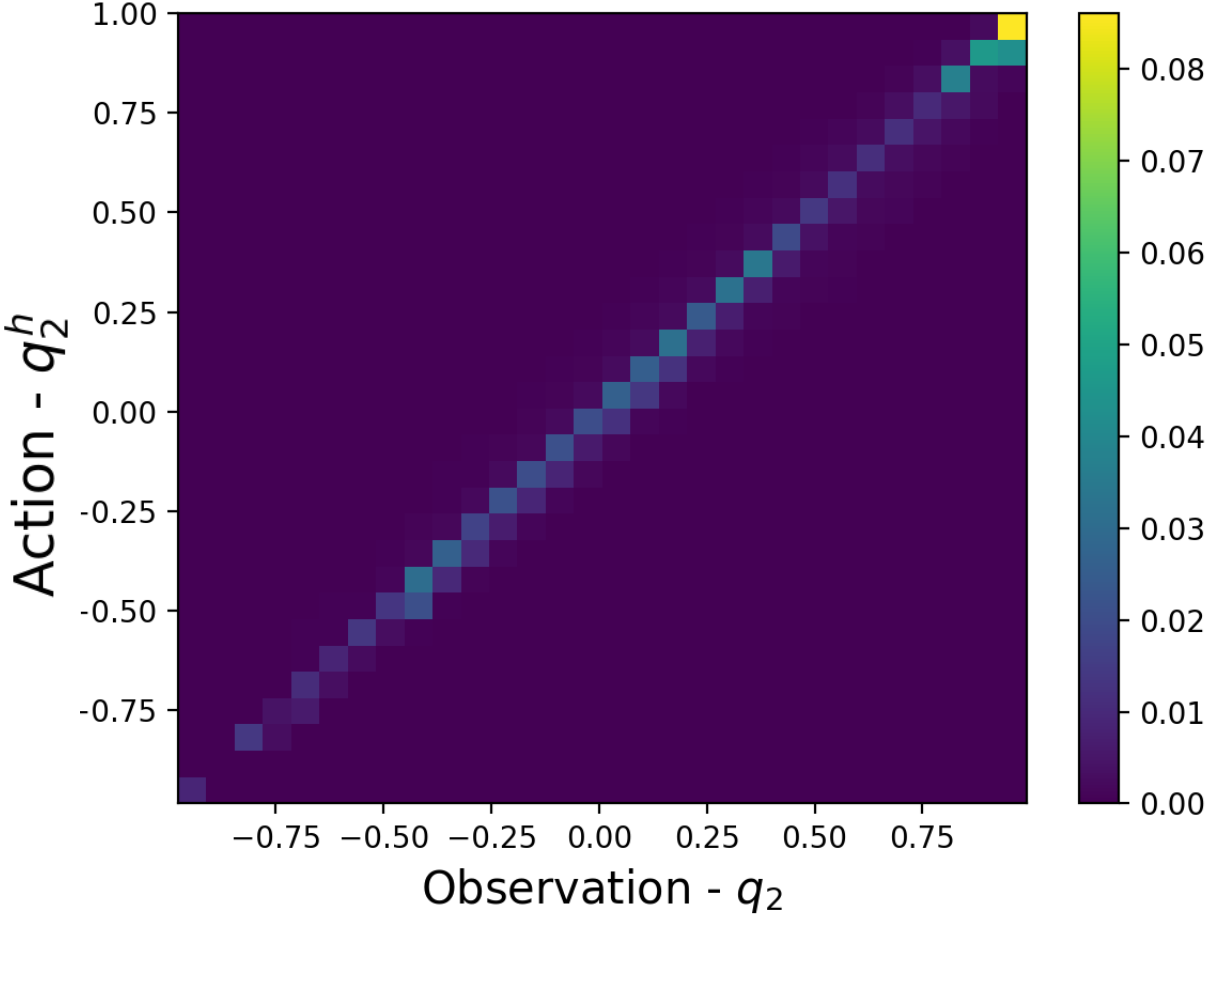
\includegraphics[width=0.3\textwidth]{figures/ch4/ch4-action-vs-observation-distribution.png}
    \caption{A joint action-observation distribution, in the simplified case where the observation is the elbow-flex actuation in a SO-100, and the action is the recorded position for the same joint from the teleoperator arm. The motion recorded being teleoperated, the points distribute along a the diagonal.}
    \label{fig:ch4-action-vs-observation-distribution}
\end{figure}

In this simplified (minimization) objective, the optimization process differs from eq.~\ref{eq:diffusion-likelihood} in that, rather than maximizing \( p_\theta \) directly, the parameters \( \theta \) of the pairwise likelihood \( p_\theta(z_{t-1} \vert z_t) \) are adjusted to \emph{predict the total displacement} \( \epsilon \) for a randomly long (\( t \sim \mathcal{U}(\{1,\dots,T\}) \)) diffusion process starting from a sample of the target distribution.

By learning the total displacement from a generally, uninformative corrupted sample obtained diffusing information and a sample from an unknown distribution~\citet{hoDenoisingDiffusionProbabilistic2020} show that one can approximate the underlying distribution reversing the displacement, \emph{denoising} samples.
Interestingly, under the hypothesis that real-world data belongs to a single, higher-dimensional manifold (Manifold Hypothesis),~\citet{permenterInterpretingImprovingDiffusion2024} show that diffusion learns the gradient of a distance function from any off-point manifold (such as perturbed, uniformative samples), and the data manifold itself.
Following this gradient---i.e., denoising a sample from an uninformative distribution---corresponds to projecting back into the manifold, yielding a procedure to sample from unknown distributions by means of Euclidean projection.
Indeed, under the assumption that \(p_\theta (z_{t-1} \vert z_t) \) is Gaussian, sampling \(z_{t-1} \sim p_\theta(\bullet \vert z_{t}) \) corresponds to computing:
\begin{align}
    z_{t-1} = \frac{1}{\sqrt{\alpha_t}} \left( z_t - \frac{\beta_t}{\sqrt{1 - \bar\alpha_t}} \epsilon_\theta(z_t, t) \right) + \sigma_t \epsilon, \quad \epsilon \sim \mathcal N(\mathbf{0}, \mathbf{I}), \label{eq:diffusion-denoising-definition}
\end{align}
thus showing that the lower-level latent variables in a DM can be obtained by iteratively removing noise from the one-step higher order variable, using the noise regressor \( \epsilon_\theta(z_t, t)\) learned minimizing eq.~\ref{eq:diffusion-simplified-loss}.

\subsubsection{Flow Matching}
\label{sec:ch4-flow-matching}
% Note: I have purposefuly avoided redefining likelihood and optimization objective for FM models as (1) I am presenting them as a generalization of DM, for which the same concepts have been presented in enough detail and (2) the derivation of the objective in the FM paper is very clear and does not really need explanation or coverage.
 
The posterior parametrization adopted by DMs proved traditionally effective, yet it raised concerns circa its \emph{efficiency} at inference time, where a possibly large number (hundreds) of compute-expensive denoising steps are needed in order to recover a sample from the target distribution.
Flow Matching (FM)~\citep{lipmanFlowMatchingGenerative2023} extends DMs to the general case of arbitrary likelihood and posteriors, and in this defines a superseding class of GMs providing a unified framework for learning \emph{continuous transformations} between distributions, encompassing and generalizing DMs.
Instead of a \emph{stochastic, discrete, multi-step} denoising process, FM aims to learn a \emph{deterministic, continuous, differentiable flow} \( \psi: [0,1] \times Z \mapsto Z \), formalized starting from a (possibly time-dependent) vector field \( v: [0,1] \times Z \mapsto Z \) \emph{transporting over time} samples from a simple prior distribution \( p_0 \)---e.g., a standard Gaussian---to a more complex, typically unknown data distribution \( p_1 \).
In this, FM accomodates for arbitrary intermediate distributions, breaking free from the particular case where posterior and likelihood are exclusively Gaussians.
Note also how FM models time \( t \in [0,1] \) to be varying continuously while moving away \emph{from} an easy-to-sample distribution \( p_0 \) \emph{towards} the unknown data-distribution, \( p_1 \).
This results in a continuous (and deterministic) trajectory at inference, which is in practice more efficient compared to following stochastic paths like in DMs.
Formally, FM can be fully characterized by an ordinary differential equation (ODE) relating instantaneous variations of flows with the underlying vector field, and hence providing complete trajectories over the distributions' support when integrating over time,
\begin{align}
    \frac{d}{dt} \psi(z, t) &= v(t, \psi(t, z)), \\
    \psi(0, z) &= z .
\end{align}
In practice, flow models learn to approximate these dynamics by estimating a vector field \( v \) that matches the true, unknown \( u \), so that the induced flows \( \psi \) can approximate the ideal trajectories \( \psi^* \).

FM proved very effective in a variety of applications, ranging from image~\citep{esserScalingRectifiedFlow2024} and video generation~\citep{polyakMovieGenCast2025} to robotics control~\citep{black$p_0$VisionLanguageActionFlow2024}.
Most notably, in their introductory work on FM for GM,~\citet{lipmanFlowMatchingGenerative2023} show how DMs can be seen as a specific instance of FM where the \emph{conditional} target vector field \( v \) learned by the noise regressor \( \eps_\theta \) corresponds to:
\begin{equation}\label{eq:fm-diffusion-vector-field}
    u(t, z\vert z_0) = \frac{\frac{d}{dt}\alpha(1-t)}{1 - (\alpha(1-t))^2}(\alpha(1-t)z - z_0), \quad \alpha(t) = e^{-\frac12 \int_0^t \beta(s) ds}, \quad \forall z_0 \in \mathcal D.
\end{equation}
Conditional vector fields are defined not only over their argument \( z \) and time \( t\), but do also vary with respect to an auxiliary variable \( z_0 \), thereby extending the standard notion of a vector field to incorporate additional conditioning.
Note that the traditional discrete-time noise-scheduler \( \{\beta_t\}_{t=0}^T \) is now generalized to a continuous map \( \beta : [0,1] \mapsto \mathbb R^+ \).
Crucially,~\citet{lipmanFlowMatchingGenerative2023} prove that by exclusively optimizing the vector field for individual data points \( z_0 \in \mathcal D \), one also retrieves the optimal flow to morph the entire support of the initial distribution \( p_0 \) into \( p_1 \ \text{s.t.} \mathcal D \sim p_1 \).


\begin{figure}
    \centering
    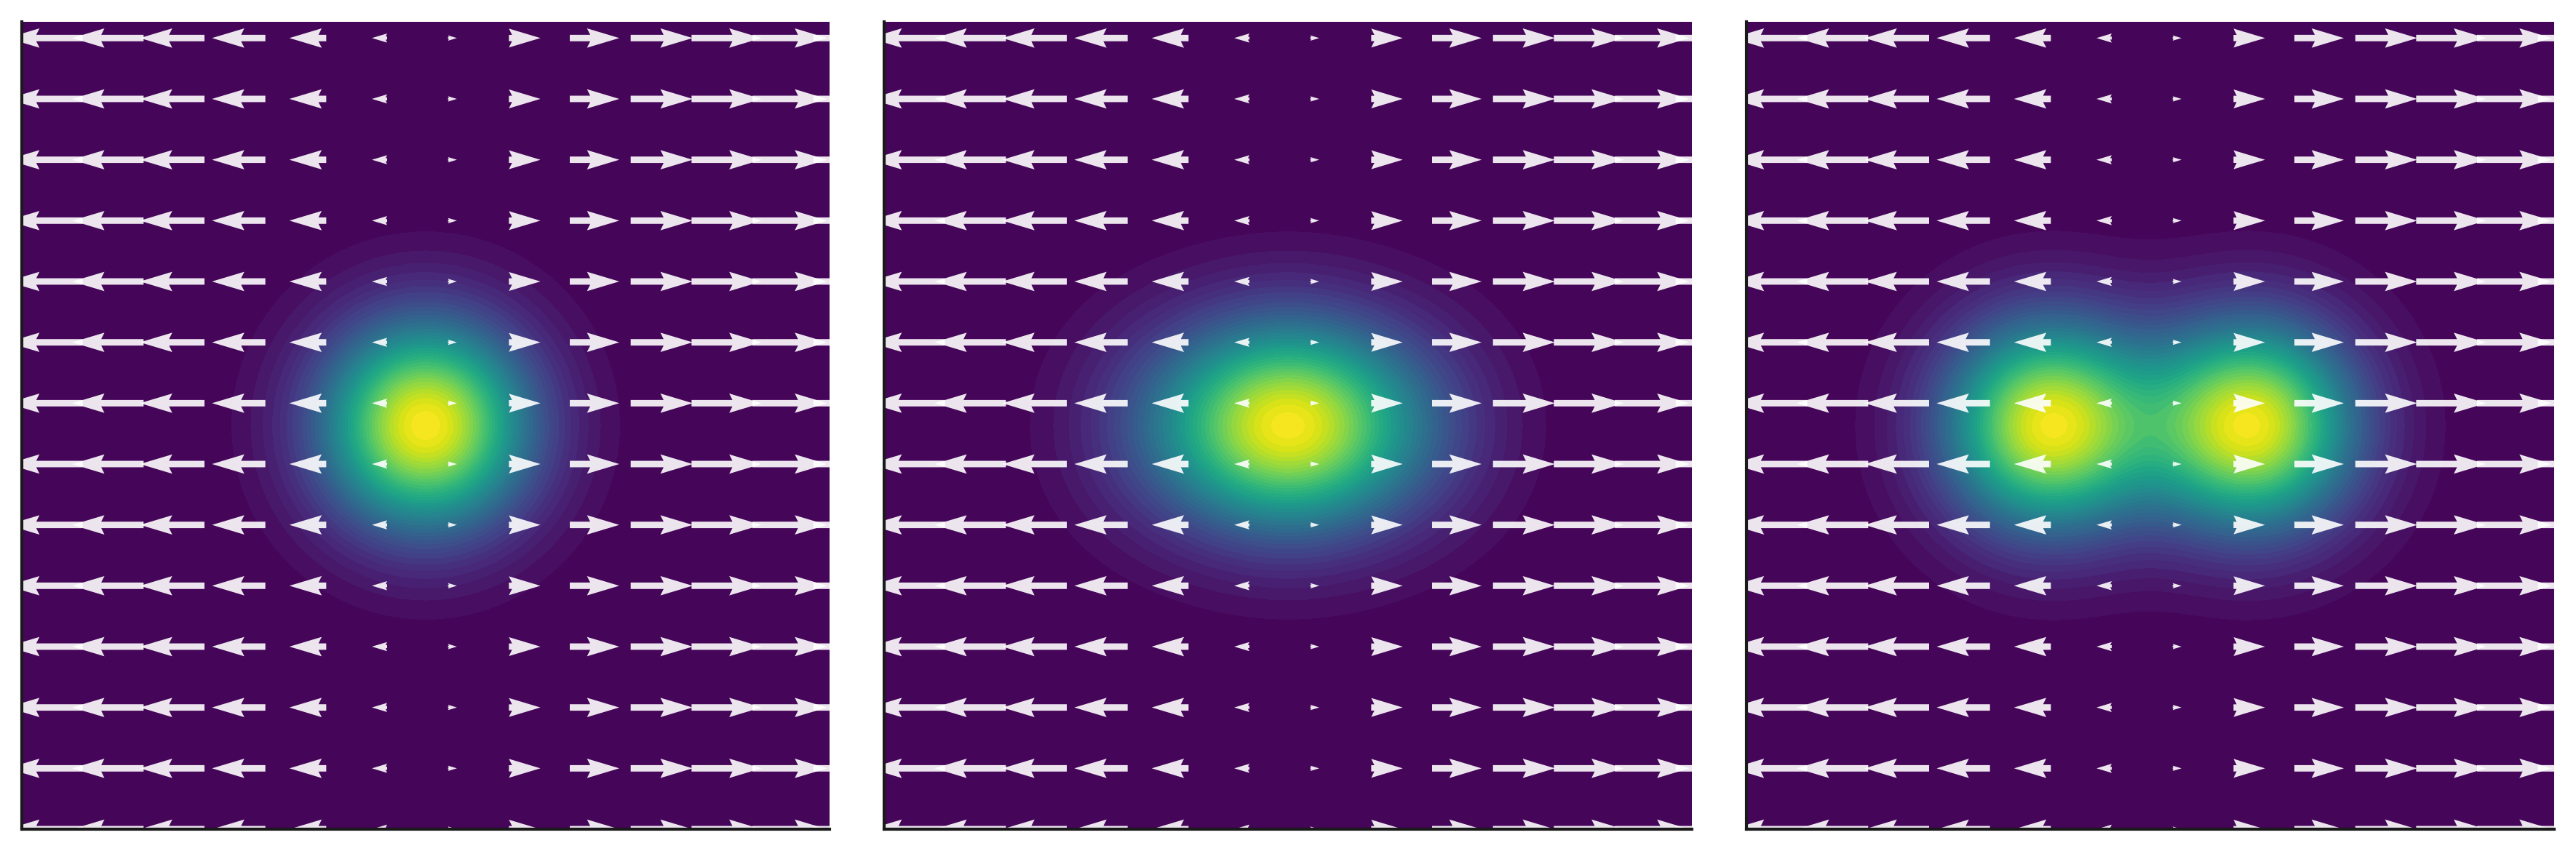
\includegraphics[width=0.9\textwidth]{figures/ch4/ch4-normalizing-flows.png}
    \caption{Probability distributions can be modified differently by applying different vector fields, inducing different flows of mass across the same support (top versus bottom, using two different time-invariant 2D-fields \( u_1(x,y) = (x,0) \) and \( u_2(x,y) = (x/\sqrt{2}, y/\sqrt{2}) \)). Notice time flows \emph{continuously} in \( [0,1] \). FM models learn to approximate a target vector field, thereby producing arbitrary (goal) transformations of an easy-to-sample initial distribution.}
    \label{fig:ch4-normalizing-flows}
\end{figure}

While the noising schedule of DMs results in a stochastic resembling a random (Brownian) walk, FM allows for more general---potentially, deterministic---likelihood and posterior parametrization.
In the FM literature the likelihood and posterior probabilty densities defined along a HMLV model are typically referred to as a \emph{probability path}, where the distributions for successive adjacent transitions in the HMLV model are related by the (normalized) flow between them (Figure~\ref{fig:ch4-normalizing-flows}).
The inherent flexibility of FM is one of their key advantages over DMs, as it opens up the possibility of \emph{learning} more efficient paths.
For instance, one can design probability paths inspired by Optimal Transport (OT), a mathematical framework concerned with characterizing the most efficient morphings between probability distributions.
Probability paths obtained through OT paths tend to be \emph{straighter} than diffusion paths (Figure~\ref{fig:ch4-diffusion-paths-versus-fm}), which can lead to faster and more stable training, as well as empirically result in higher-quality generations with fewer denoising steps at inference time.
In particular, by avoiding unnecessary backtracking associated with the inherent stochastic nature of both the noising and denoising process in DMs, test-time compute is typically significantly reduced in FM, while retaining comparable results~\citep{lipmanFlowMatchingGenerative2023}.

\begin{figure}
    \centering
    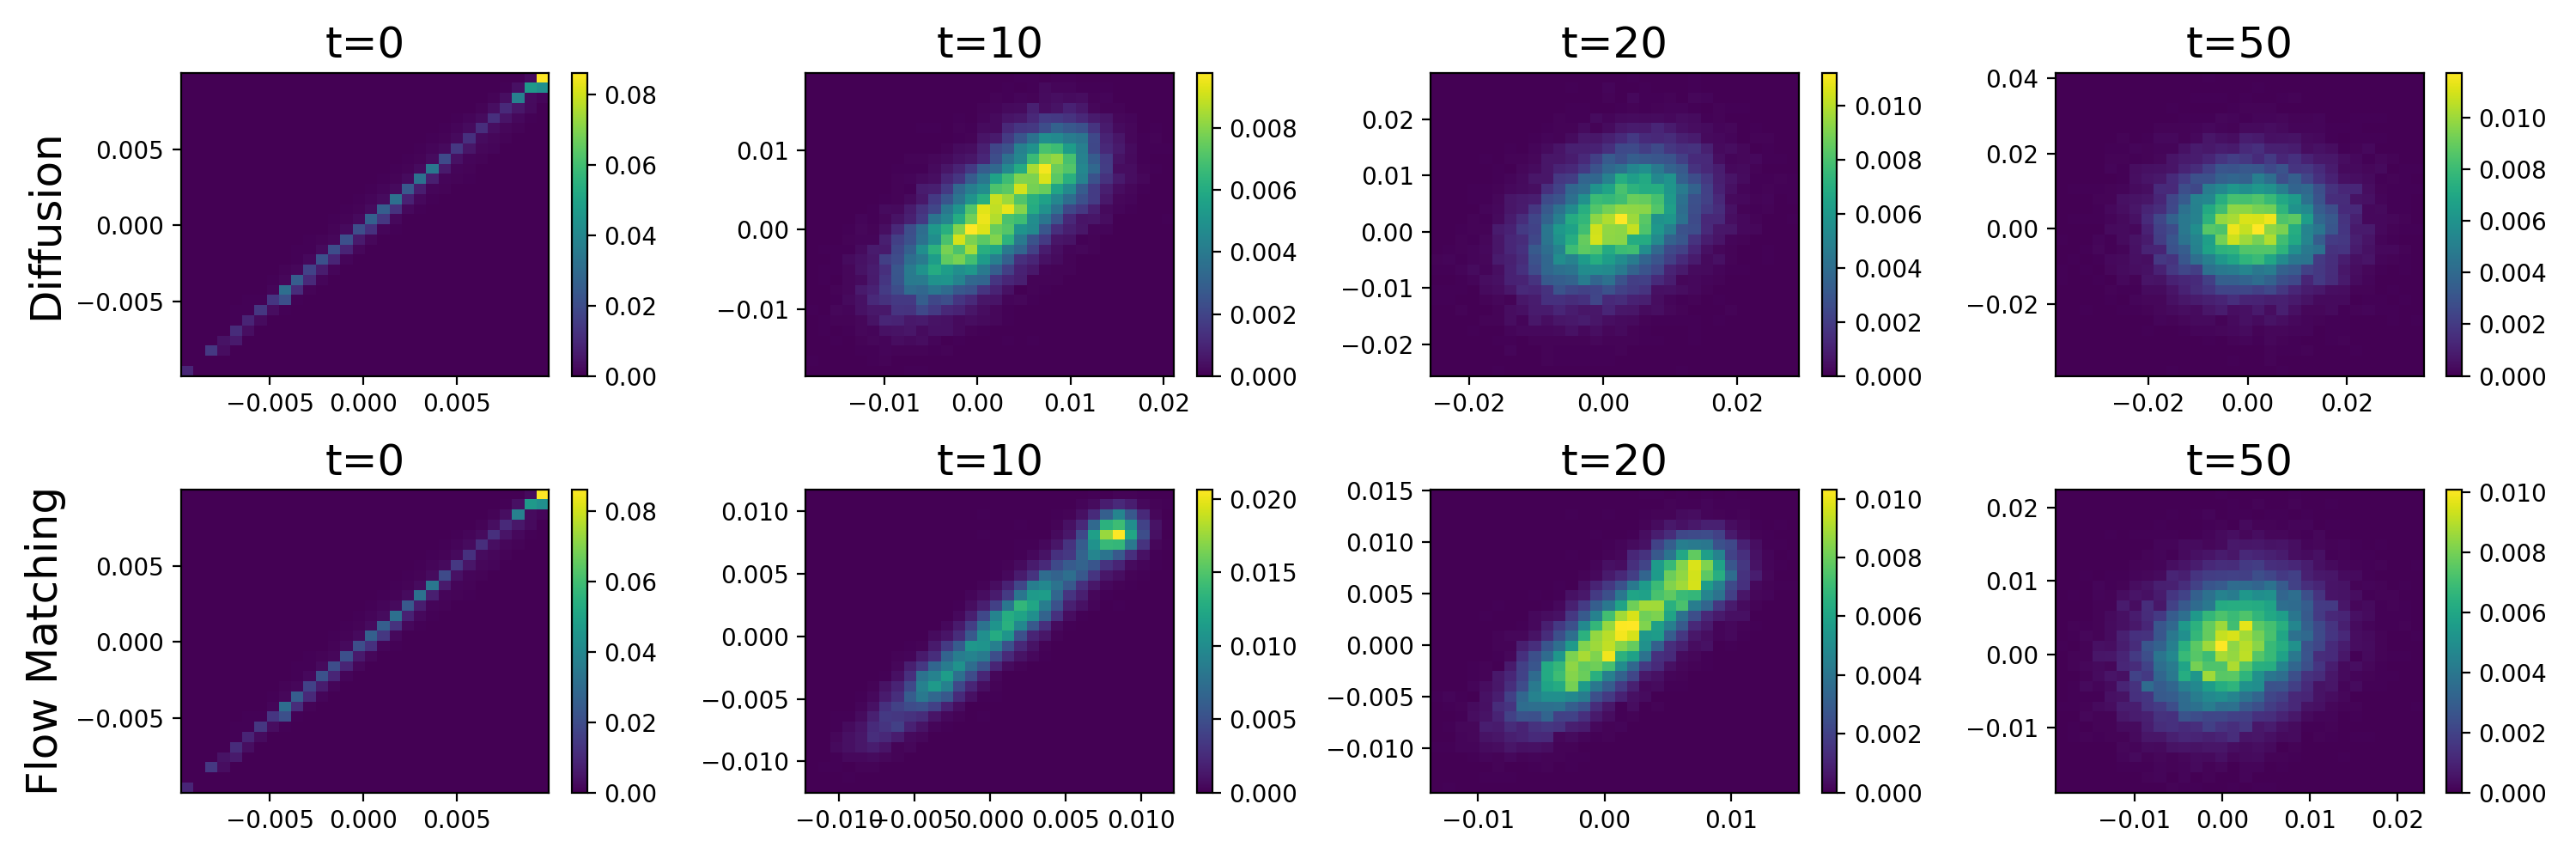
\includegraphics[width=\textwidth]{figures/ch4/ch4-diffusion-vs-flowmatching.png}
    \caption{Compared to diffusion, flow matching distorts distribution along a less randomic pattern, resulting in a clearer interpolation between source and target distribution. The visualization shows an example comparison between these two methods on joint distribution of robot observations and actions over \( T=50 \) steps.}
    \label{fig:ch4-diffusion-paths-versus-fm}
\end{figure}


In practice, FM can be applied to generative modeling by learning a vector field regressor \( v_\theta(z, t) \) to approximate a given target vector field \( u(t, z) \).
In the particular case of DMs, \( u(t, z) \) is defined as in eq.~\ref{eq:fm-diffusion-vector-field}, while in priciple the target vector field can be learned to induce an arbitrary mass displacement, or fixed according to OT.
Given a sample from the data distribution \( z_1 \sim p_1 \) and a sample from an easy-to-sample prior \( z_0 \sim p_0 \), Conditional FM (CFM) defines a simple path between them using \emph{linear interpolation} between samples \( z_t = (1-t)z_0 + t z_1 \), which in turn results in the target vector field \( u(t, z_t) = z_1 - z_0 \).
FM models can then be trained with a simple regression objective defined as:
\begin{align}\label{eq:flow-matching-objective}
    \mathcal L(\theta) = \mathbb{E}_{t, z_0, z_1} \big[
        \Vert v_\theta((1-t)z_0 + t z_1, t) - (z_1 - z_0) \Vert^2 \big], \quad t \sim \mathcal{U}([0,1]),
\end{align}
where \( z_0 \sim p_0(\bullet) \) and \( z_1 \sim p_1(\bullet) \). 
Note how in eq.~\ref{eq:flow-matching-objective}---differently from eq.~\ref{eq:diffusion-simplified-loss}---time is assumed to be varying continuously \( t \sim \mathcal U([0,1]) \) rather than discretely \( t \sim \mathcal U(\{0, \Delta t, 2 \Delta t, \dots, 1 \})\), a key property of flow-based models.
Therefore, the objective in eq.~\ref{eq:flow-matching-objective} directly regresses the learned vector field onto the simple, straight path connecting a point from the prior and a point from the data, providing a simulation-free training procedure that is both stable and efficient.
At inference time, samples are generated by starting with \( z_0 \sim p_0 \) and iteratively refined according to \( \frac{dz}{dt} = v_\theta(z_t, t) \) for \(t \in [0,1] \)---an operation that can be numerically carried out with standard ODE solvers, and that in practice is often carried out numerically via forward-Euler integrating over tens of denoising steps.

\subsection{Action Chunking with Transformers}
While GMs prove useful in learning complex, high-dimensional multi-modal distributions, they do not natively address the compouding errors problem characteristic of modeling online, sequential predictions.
In Action Chunking with Transformers (ACT),~\citet{zhaoLearningFineGrainedBimanual2023} present an application of VAEs to the problem of learning purely from offline trajectories, and introduce a simple, yet effective method to mitigate error compounding, learning high-fidelity autonomous behaviors via BC.
Drawing inspiration from how humans plan to enact \emph{sequences} of actions \( a_{t:t+k} \) instead of single actions \( a_t \),~\citet{zhaoLearningFineGrainedBimanual2023} propose learning a GM on a dataset of input demonstrations by modeling \emph{chunks} of multiple actions directly.
Besides contributions to learning high-performance autonomous behaviors,~\citet{zhaoLearningFineGrainedBimanual2023} also introduce hardware contributions in the form of a low-cost bimanual robot setup (ALOHA) capable of performing fine-grained manipulation tasks, such as opening a lid, slotting a battery in its allotment or even prepare tape for application.
Notably, ALOHA bimanual setup costs just as much as a mono-arm Franka arm and can be assembled from easy-to-source parts, underscoring its higher accessibility.

\citet{zhaoLearningFineGrainedBimanual2023} do also present significant algorithmic contributions related to synthetizing performant autonomous behaviors for the ALOHA setup, adopting transformers as the architectural backbone to learn a \emph{Conditional} VAE~\citep{sohnLearningStructuredOutput2015} from demonstrations. 
Conditional VAEs are a variation of the standard VAE  introducing an arbitrary conditioning on sampling from the latent prior, modeling \emph{one-to-many} relationships between latent and data samples.
Further, in stark contrast with previous work~\citep{florenceImplicitBehavioralCloning2022,jannerPlanningDiffusionFlexible2022},~\citet{zhaoLearningFineGrainedBimanual2023} do not learn a full joint \( p_\theta(o,a) \) on observation and actions, and rather focus on the conditional \( p_\theta(a \vert o) \).
While the \emph{policy} distribution \( p_\theta(a \vert o) \) can in principle be entirely described from the joint \( p_\theta(o,a) \), conditional distributions are often intractable when using function approximators, as \( p_\theta(a \vert o) = \tfrac{p_\theta(o,a)}{\int_\actionspace p_\theta(o,a)} \), and the integral in the denominator is typically intractable.
Thus, instead of modeling the full joint using a vanilla VAE,~\citet{zhaoLearningFineGrainedBimanual2023} propose learning a \emph{conditional} VAE~\citep{sohnLearningStructuredOutput2015} modeling the policy distribution directly, hence approximating \( p (a \vert o) \).

In practice, when learning from demonstrations adopting CVAEs results in a slight modification to the VAE objective in eq.~\ref{eq:ELBO}, which is adapted to:
\begin{align}\label{eq:c-ELBO}
    \text{ELBO}_{\mathcal D}(\theta, \phi, \omega) = \sum_{i=0}^{N} \left(
            \mathbb{E}_{z \sim q_\phi(\cdot \vert o_i, a_i)} \big[ \log p_\theta(a_i \vert z, o_i) \big]
        - \DKL \big[ q_\phi(z \vert o_i, a_i) \Vert p_\omega(z \vert o_i) \big]
        \right)
\end{align}
Notice how in eq.~\ref{eq:c-ELBO} we are now also learning a new set of parameters \( \omega \) for the prior distribution in the latent space.
Effectively, this enables conditioning latent-space sampling (and thus reconstruction) during training (and potentially inference too), providing useful when learning inherently conditional distributions like policies.
Further, ACT is trained as a \( \beta\)-CVAE~\citep{higgins2017beta}, weighing the KL regularization term in eq.~\ref{eq:c-ELBO} with an hyperparameter \( \beta \in \mathbb R^+ \) regulating the information condensed in the latent space, where \emph{higher} \( \beta \) results in a \emph{less} expressive latent space.

In their work,~\citet{zhaoLearningFineGrainedBimanual2023} ablated using a GM to learn from human demonstrations compared to a simpler, supervised objective, \( \mathcal L_1(a,a^\prime) = \Vert a - a^\prime \Vert_1 \).
Interestingly, they found the performance of these two approaches to be comparable when learning from \emph{scripted} demonstrations. 
That is, when learning from data collected rolling out a predetermined set of commands \( [q^c_0, q^c_1, \dots] \), GM did \emph{not} prove competitive compared to standard supervised learning.
However, when learning from human demonstrations---i.e., from data collected executing commands coming from a human controller \( [q^h_0, q^h_1, \dots] \)---~\citet{zhaoLearningFineGrainedBimanual2023} found performance (defined as the success rate on a downstream task) to be severily (-33.3\%) hindered from adopting a standard supervised learning objective compared to a richer, potentially more complex to learn variational objective.
The result of such ablation reflects from the multimodal nature of human demonstrations data, and is consistent with the findings presented by~\citet{florenceImplicitBehavioralCloning2022}.
The authors also ablate the action chunking paradigm, reporting significant performance gains deriving from using action chunking (1\% vs. 44\% success rate).
To reduce acting open-loop,~\citet{zhaoLearningFineGrainedBimanual2023} also design an inference process consisting in performing inference at every timestep \( t \) and then aggregate multiple chunks using an exponential moving average (EMA) on the overlapping chunks.

In ACT (Figure~\ref{fig:ch4-act}), inference for a given observation \( o \in \mathcal O \) could be performed by (1) defining a prior \( p_\omega(z \vert o) \) for the latent variable \( z \) and (2) decoding an action chunk from a sampled latent \( z \sim p_\omega(\bullet \vert o) \), similarily to how sampling from standard VAEs takes place, with the exception that vanilla VAEs typically pose \( p(z\vert o) \equiv p(z) \sim \mathcal N(\mathbf{0}, \mathbf{I}) \) and thus skip (1).

\begin{figure}
    \centering
    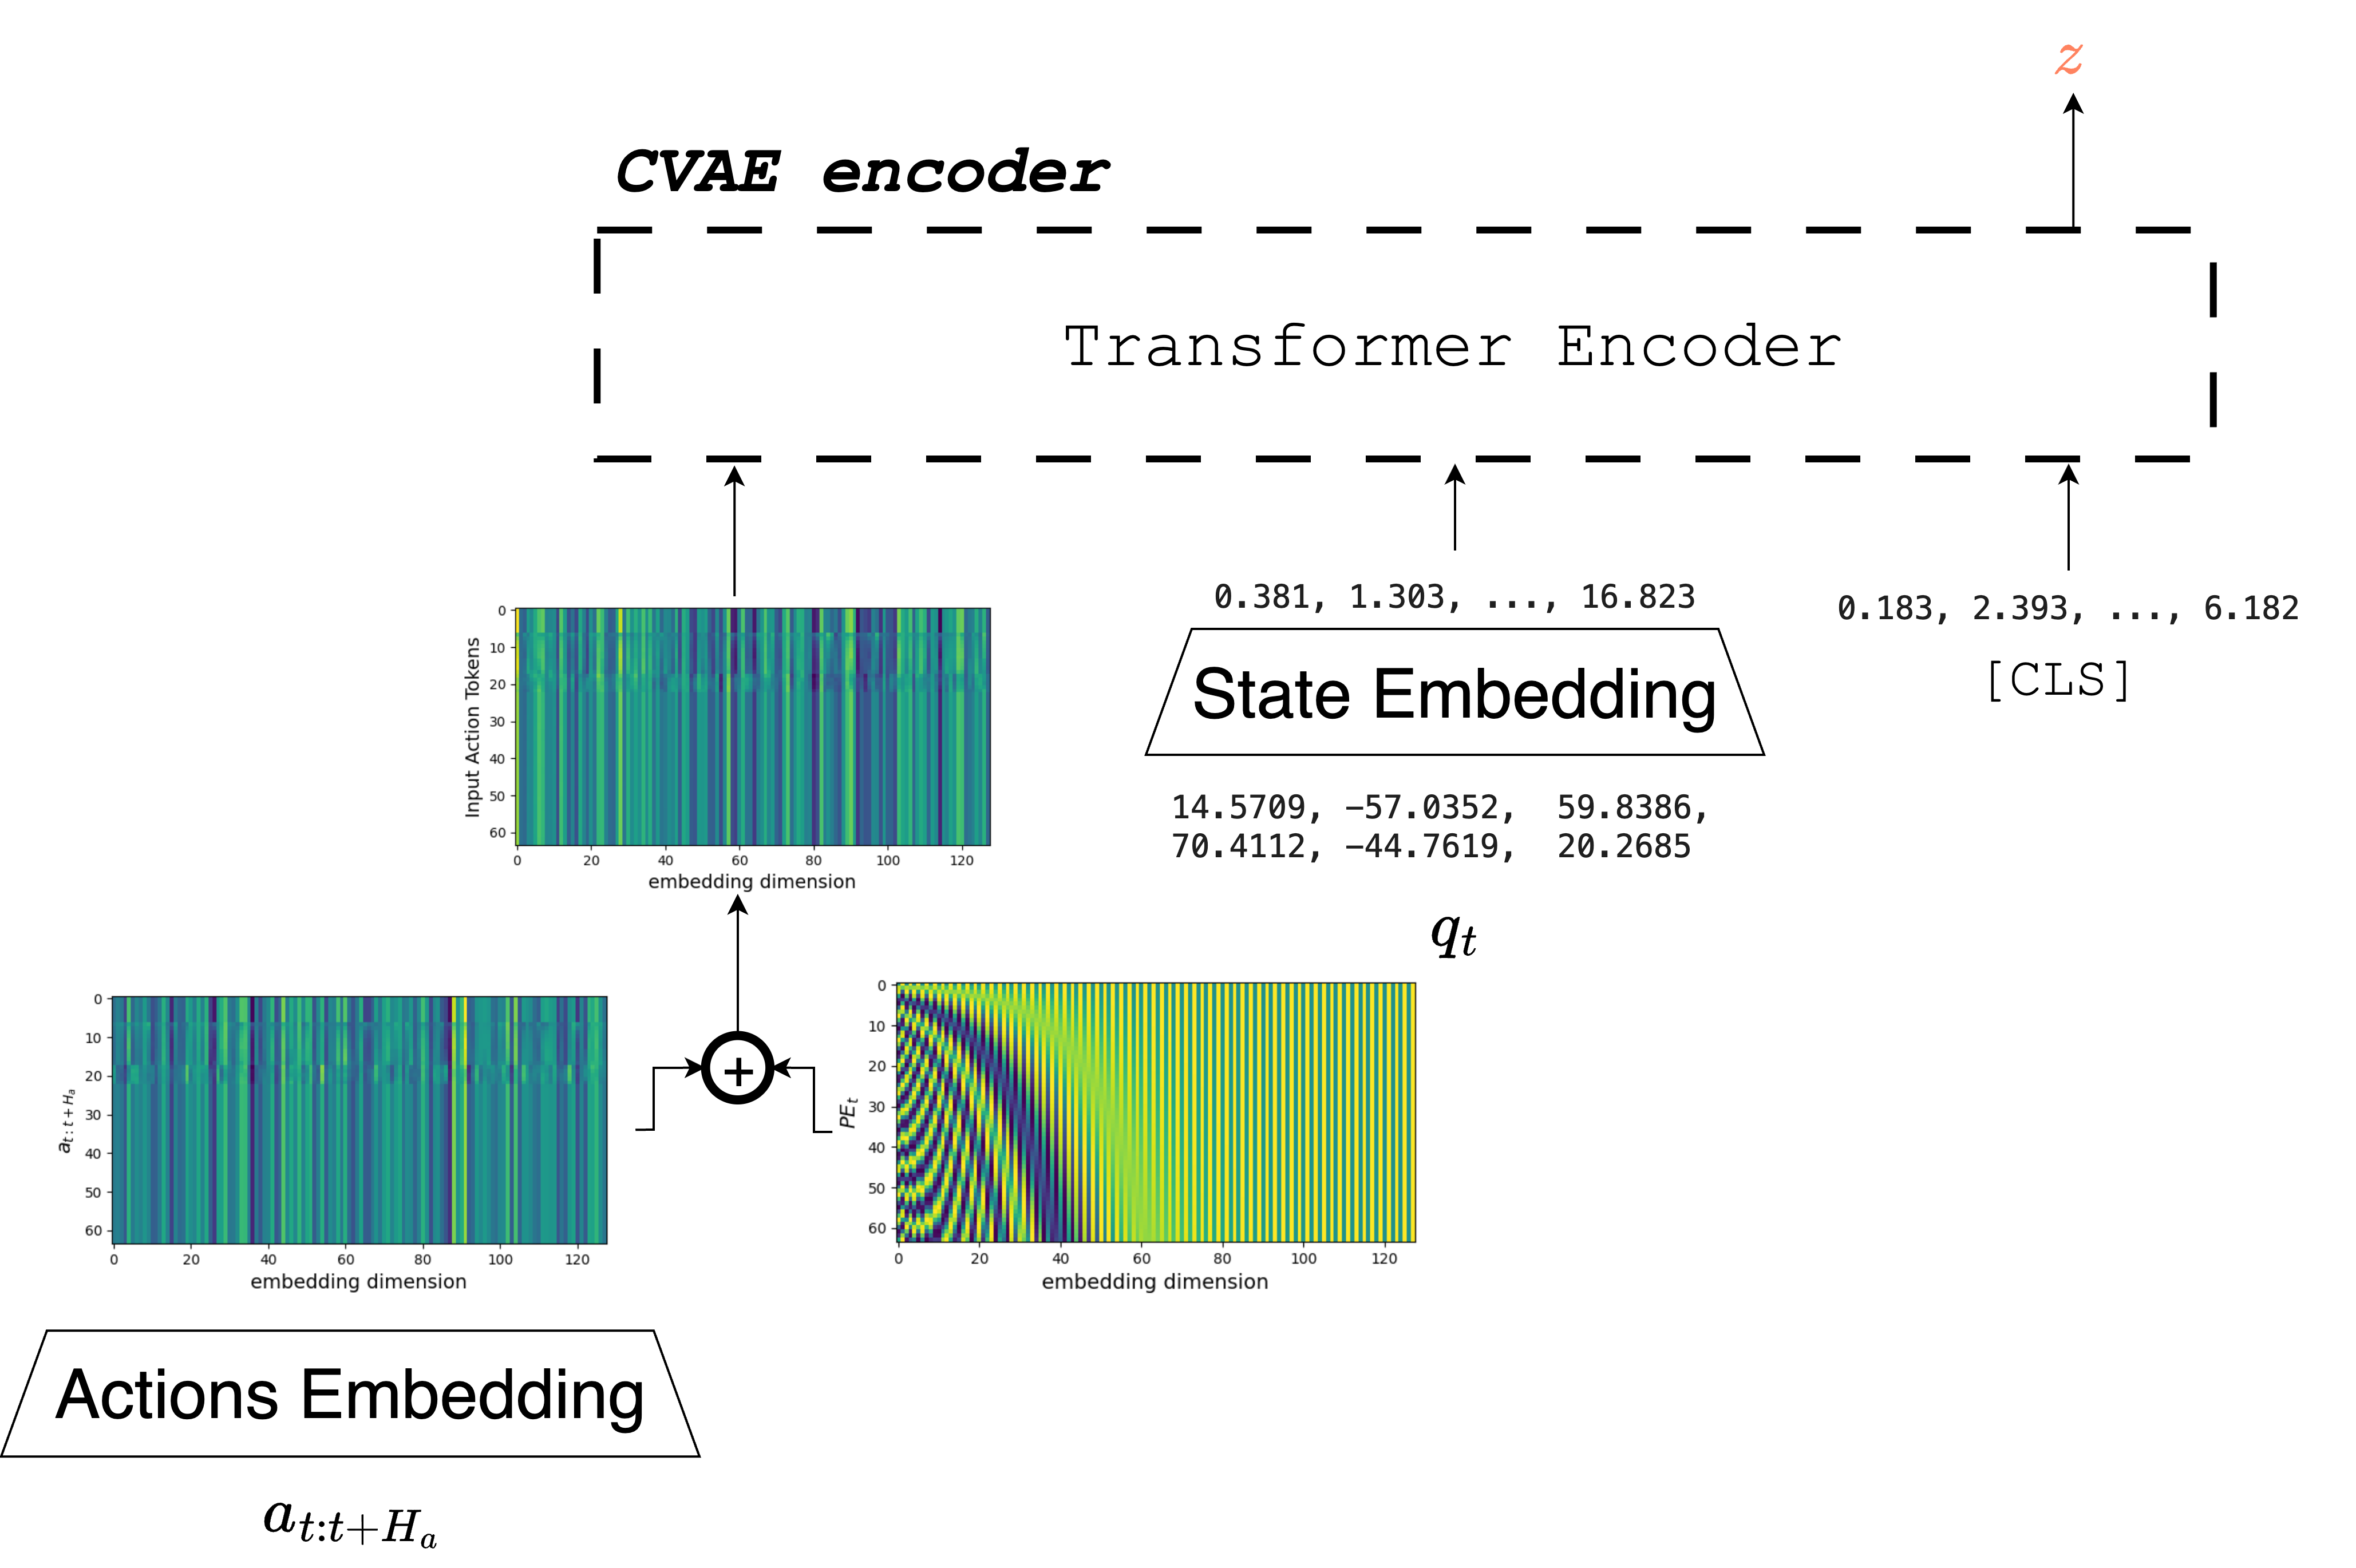
\includegraphics[width=0.75\textwidth]{figures/ch4/ch4-act-encoder.png}
    \caption{The CVAE encoder used in ACT. Input action chunks are first embedded and aggregated with positional embeddings, before being processed alongside embedded proprioperceptive information, and a learned \texttt{[CLS]} token used to aggregate input level information, and predict the style variable \( z \). The encoder is exclusively used to \emph{train} the decoder, and it is entirely disregarded at inference time.}
    \label{fig:ch4-act-encoder}
\end{figure}

However, the authors claim that using a deterministic procedure to sample \( z \) benefits policy evaluation, and thus avoid using the conditional prior at all at inference time, effectively using the CVAE framework exclusively to train a more expressive decoder.
At test time,~\citet{zhaoLearningFineGrainedBimanual2023} propose simply using \( z = \mathbf{0} \), as the conditional prior on \( z \) used in training is set to be a standard Gaussian.
Further, conditioning on the observation \( o \) is achieved through explicitly feeding proprioperceptive and visual observations to the decoder, \( p_\theta(a \vert z, o) \) at test time.
If at inference \( z \) is sampled from a standard Gaussian, during training \( z \) is sampled from an approximate posterior distribution \(q_\phi(z \vert o, a)\), which, however, disregards image observations and exclusively uses proprioperceptive states to form \( o \) for efficiency reasons.

\begin{figure}
    \centering
    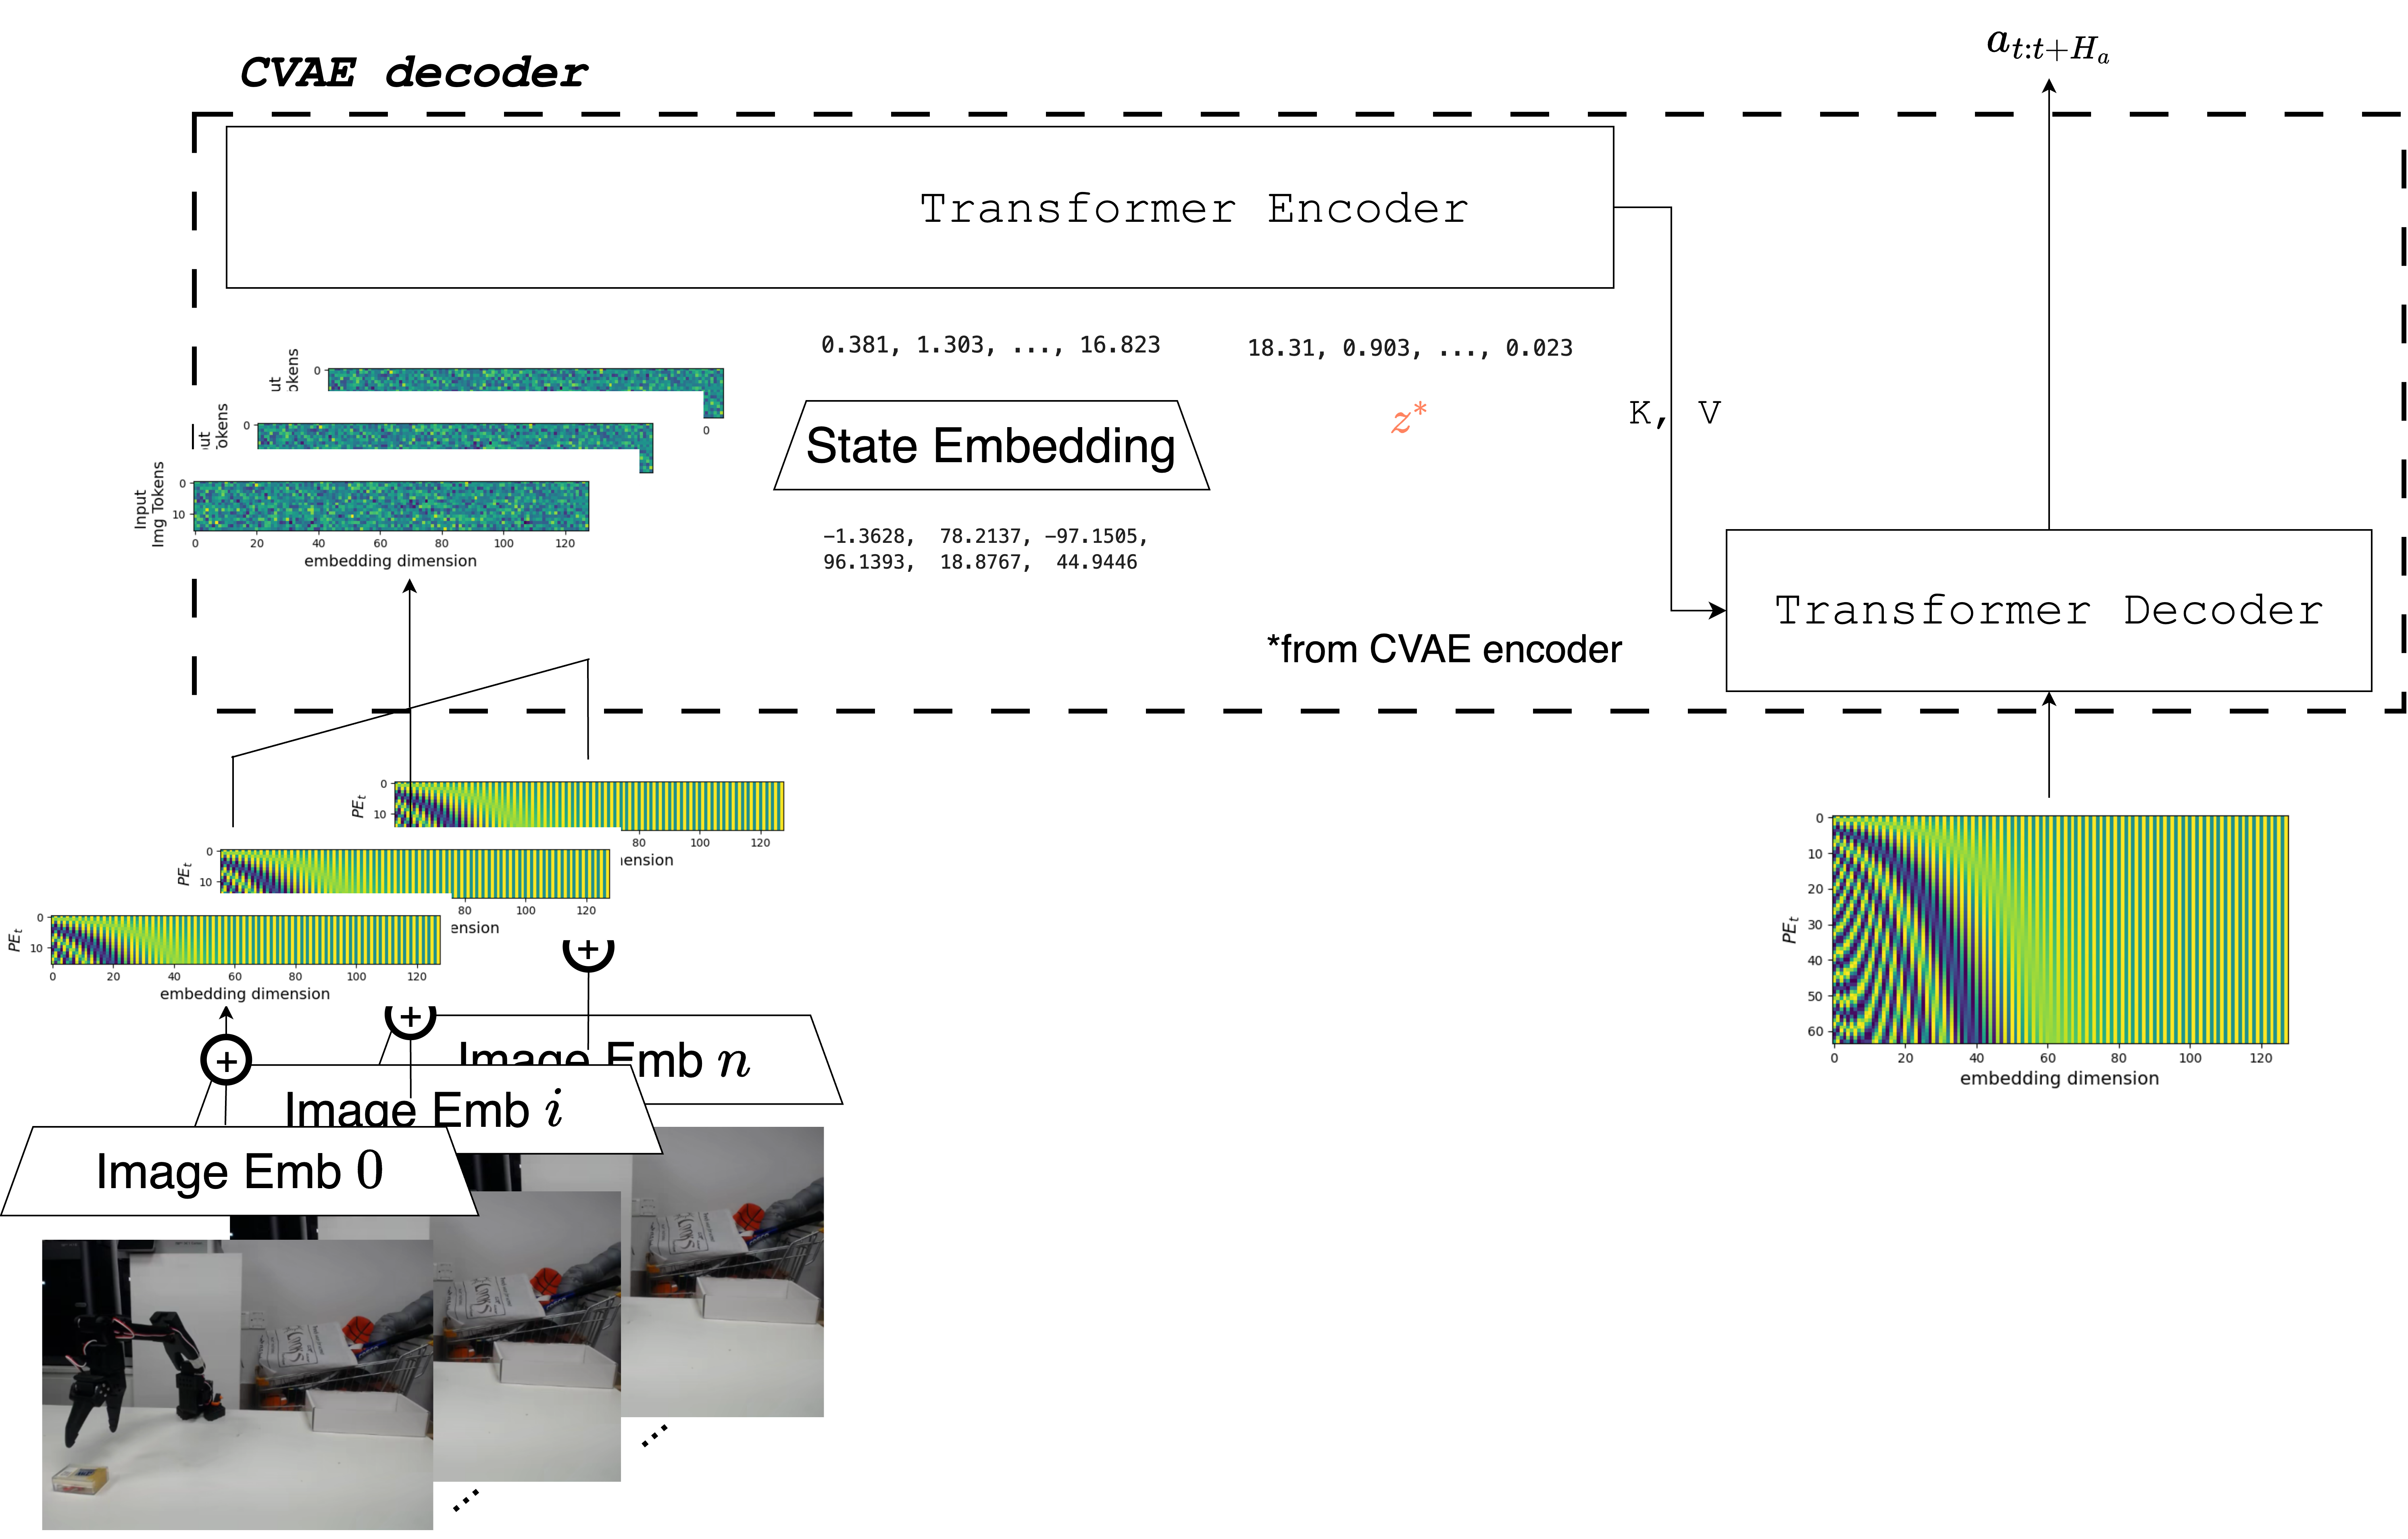
\includegraphics[width=0.75\textwidth]{figures/ch4/ch4-act-decoder.png}
    \caption{The CVAE decoder used in ACT, comprising of a full encoder-decoder Transformer architecture. Camera observations from all \( n \) camera views are first embedded using pre-trained visual encoders, and then aggregated with the corresponding positional embeddings. Then, the proprioperceptive information and style variable \( z \) retrieved from the CVAE encoder, are fed to the encoder-decoder Transformer for inference. The encoder shares the matrices \( K,V \) with the decoder, and is trained to decode fixed position embeddings into action chunks.}
    \label{fig:ch4-act-decoder}
\end{figure}

\subsubsection{Code Example: Training and Using ACT in Practice}

\begin{figure}
    \centering
    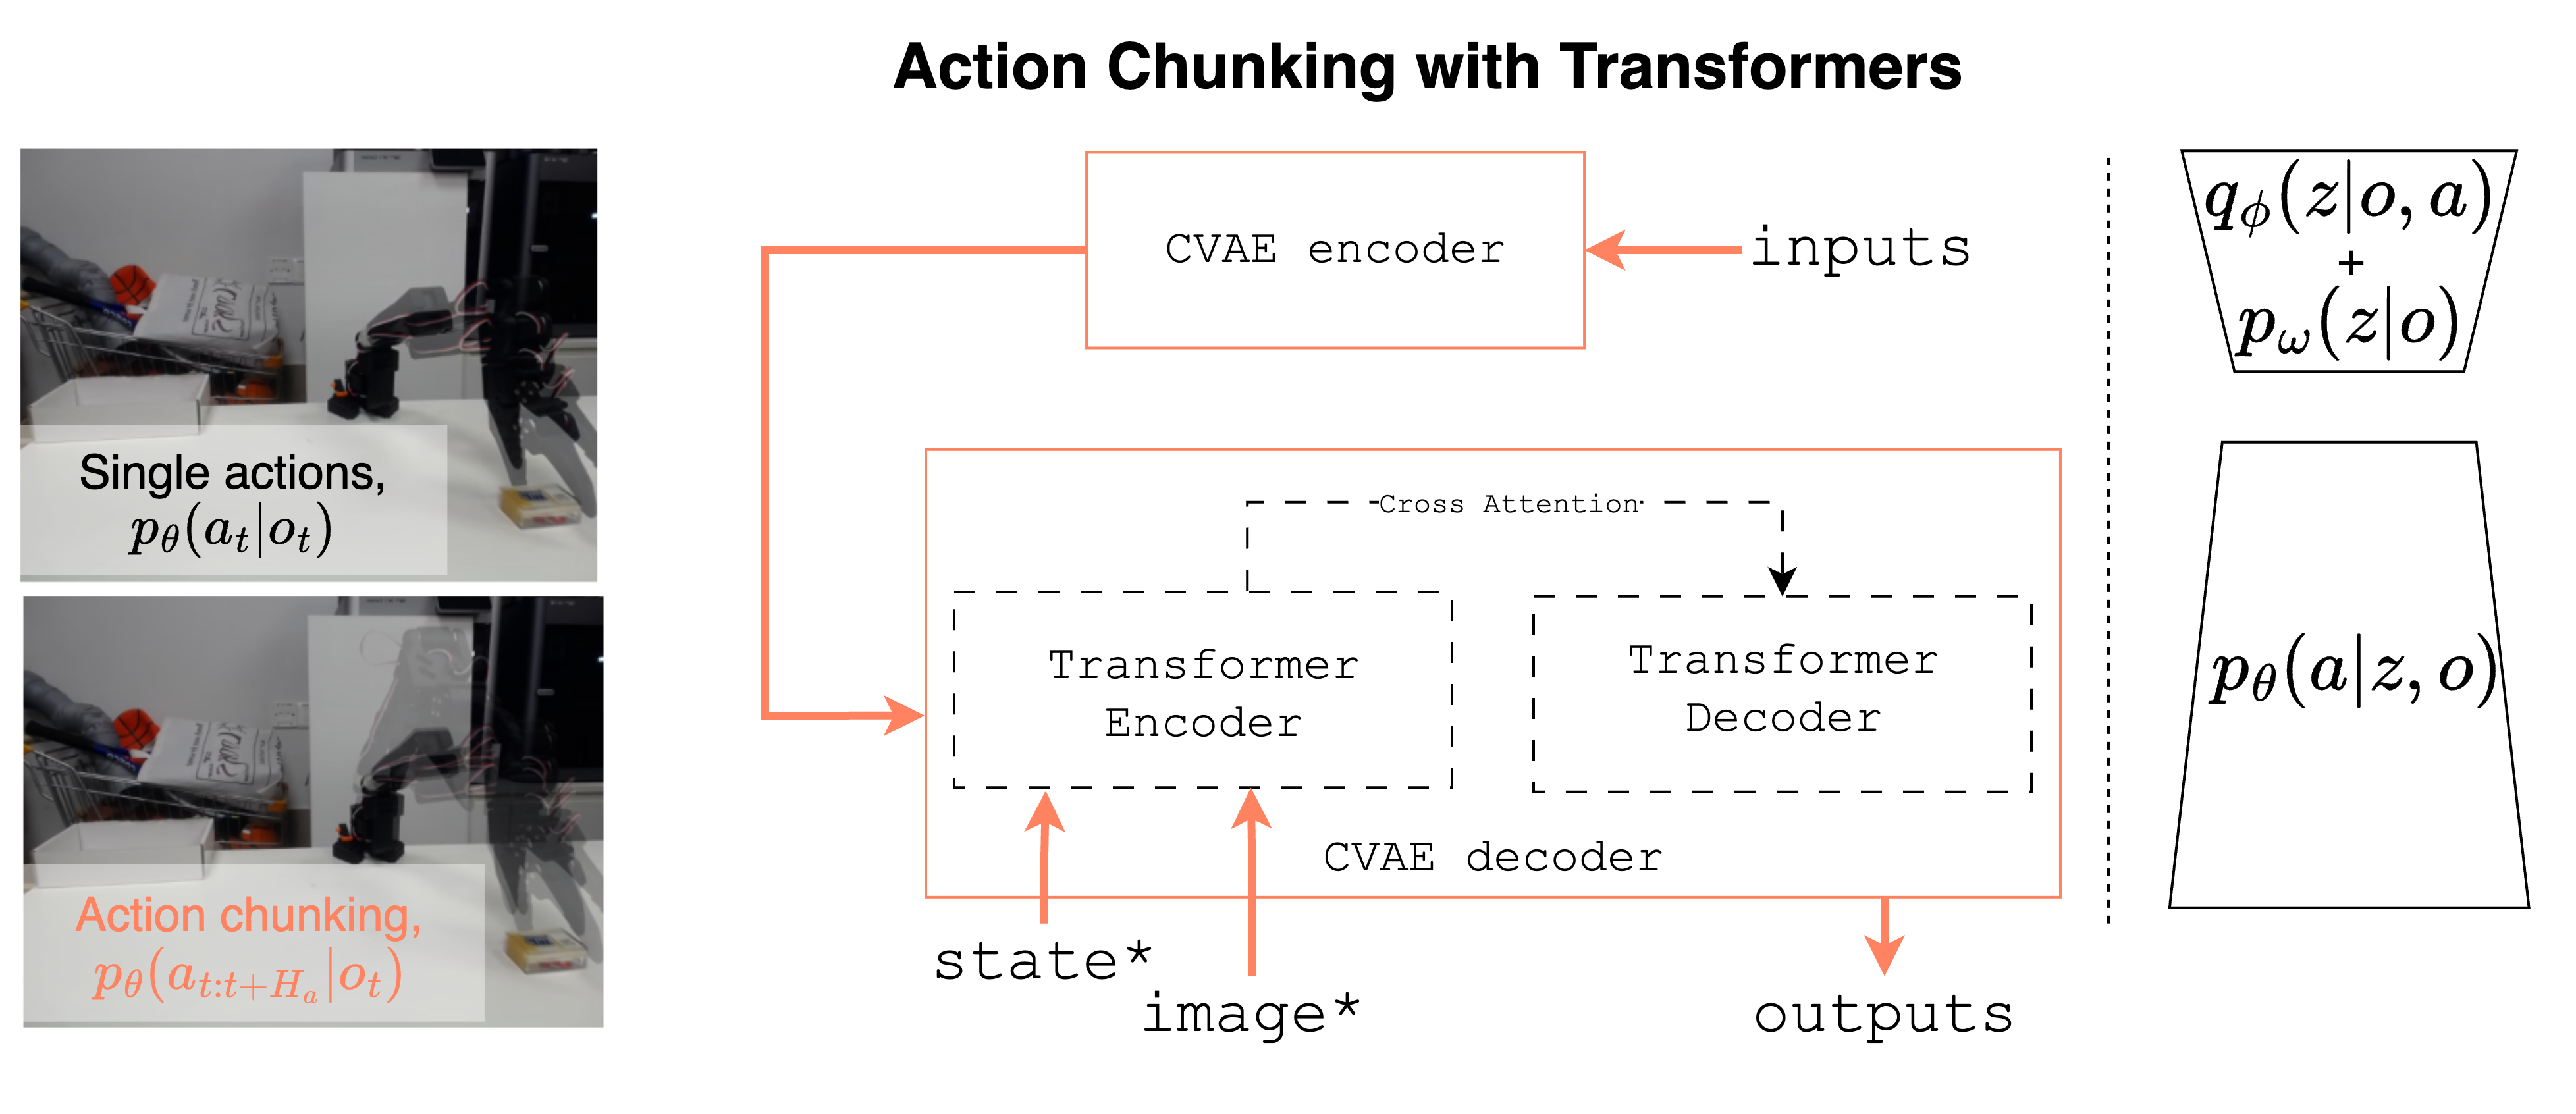
\includegraphics[width=0.9\textwidth]{figures/ch4/ch4-act.png}
    \caption{Action Chunking with Transformer (ACT), as in~\citet{zhaoLearningFineGrainedBimanual2023}. ACT introduces an action chunking paradigm to cope with high-dimensional multi-modal demonstration data, and a transformer-based CVAE architecture.}
    \label{fig:ch4-act}
\end{figure}

% \paragraph{Training ACT}
\begin{pbox}[label={ex:act_training}]{Training ACT}
    \inputminted{python}{snippets/ch4/01_training_act.py}
\end{pbox}

% \paragraph{Using ACT}
\begin{pbox}[label={ex:act_using}]{Using ACT}
    \inputminted{python}{snippets/ch4/02_using_act.py}
\end{pbox}

\subsection{Diffusion Policy}
DMs have proven very effective in approximating complex highly dimensional distributions, such as distributions over images~\citep{hoDenoisingDiffusionProbabilistic2020} or videos~\citep{polyakMovieGenCast2025}, thanks to their inherent capability to deal with multimodal data, and their training stability.
In Diffusion Policy (DP),~\citet{chiDiffusionPolicyVisuomotor2024} present an application of DMs the field of robot learning, leveraging diffusion to model expert demonstrations in a variety of simulated and real-world tasks.
Similarily to ACT~\citep{zhaoLearningFineGrainedBimanual2023},~\citet{chiDiffusionPolicyVisuomotor2024} (1) adopt a modified \emph{observation-conditioned target distribution} instead of the full joint \( p(o,a) \), and (2) predict multiple actions into the future instead of a single action.
Besides the intractability of the observations' marginal \( p_\theta(o) \) given \(p_\theta(o,a) \), DP's choice to model the data distribution through \( p_\theta(a \vert o) \) also stems from the computational burden of diffusion at test time: generating actions together with observations would require a large number of denoising steps—an unnecessarily slow and ultimately unhelpful process, given that robotics focuses on producing controls rather than reconstructing observations.

In practice, conditioning on observation data is achieved conditioning the noise regressor \( \epsilon_\theta \) introduced in eq.~\ref{eq:diffusion-simplified-loss} on a stack of \( H_o \) observations, resulting in the \emph{conditional}, simplified diffusion objective:
\begin{align}
    \mathcal L(\theta) &= \mathbb{E}_{t, a_{t:t+H_a}, \epsilon} \big[
        \Vert \epsilon - \epsilon_\theta(\sqrt{\bar \alpha_t} a_{t:t+H_a} + \epsilon \sqrt{1 - \bar \alpha_t}, t, o_{t-H_o:t}) \Vert^2 \big], \label{eq:diffusion-policy-objective} \\
        & t \sim \mathcal{U}(\{1,\dots,T\}), \quad
        a_{t:t+H_a}, o_{t-H_o:t} \sim \mathcal{D}, \quad
        \epsilon \sim \mathcal{N}(\mathbf{0},\mathbf{I}). \notag 
\end{align}
Note how in eq.~\ref{eq:diffusion-policy-objective} the noise regressor is conditioned on both the latent variable rank \( t \) \emph{and} on a stack of previous observations \(o_{t-H_o:t} \).
\citet{chiDiffusionPolicyVisuomotor2024} claim the combination of (1) conditioning on a horizon of previous observations and (2) predicting multiple actions into the future allows DP to \emph{commit to specific modes} in the data at inference time, which proves essential for good performance and avoiding undecisiveness.

\begin{figure}
    \centering
    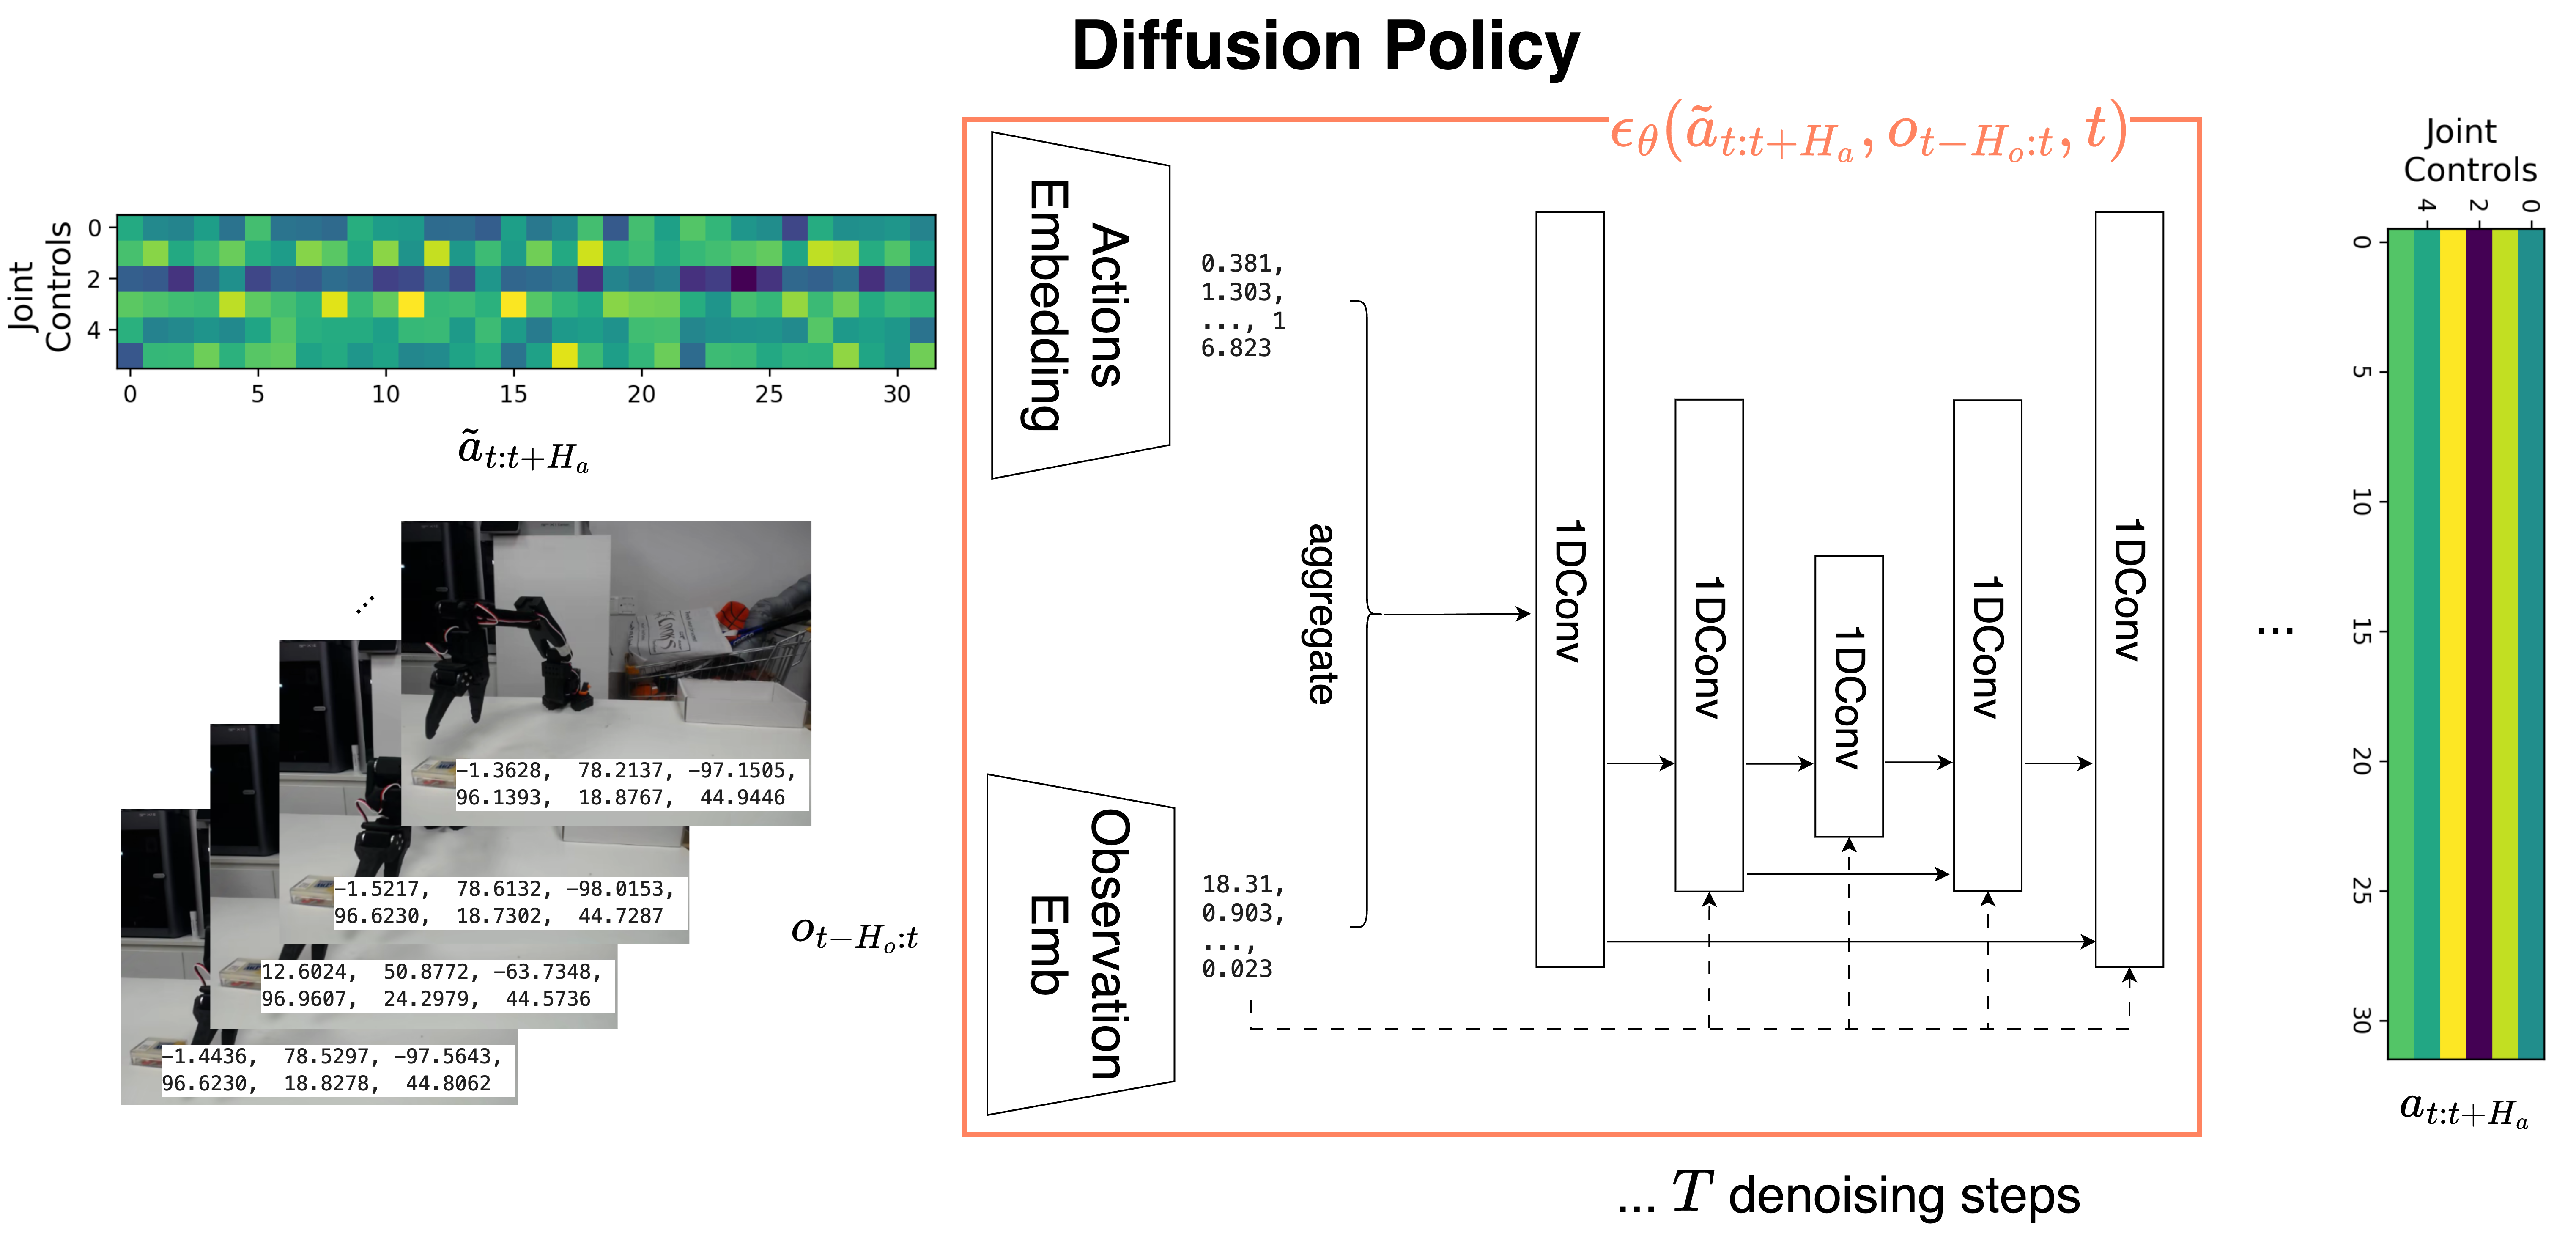
\includegraphics[width=0.9\textwidth]{figures/ch4/ch4-diffusion-policy.png}
    \caption{The Diffusion Policy archicture, as in~\citet{chiDiffusionPolicyVisuomotor2024}. A stack of \( H_o \) previous observations is used as external conditioning to denoise a group of \( H_a \) actions. Conditioning is performed at every layer of a U-Net block. Diffusion Policy allows to obtain fully-formed action chunks with as little as \(T=10\) denoising steps.}
    \label{fig:diffusion-policy-architecture}
\end{figure}

Figure~\ref{fig:diffusion-policy-architecture} shows the convolution-based version of the architecture proposed by~\citet{chiDiffusionPolicyVisuomotor2024}, illustrating inference on a single sample drawn from \( \mathcal D \), for simplicity.
The starting, arbitrarily noisy chunk of \( H_a \) actions \(\tilde a_{t:t+H_a} \) is first mapped to a (learned) high-dimensional space.
Similarily, both image observations and poses are also embedded before being aggregated to the action embeddings.
Then, a U-Net~\citep{ronnebergerUNetConvolutionalNetworks2015} is trained to regress the noise added into \( \tilde a_{t:t+H_a} \), conditioned on observation information at every layer, thus seeking to optimize eq.~\ref{eq:diffusion-policy-objective}.
At inference time, the noise predictor is used to predict the quantity of noise at every \( t \in [T, \dots, 0 ] \) and iteratively subtract it from \(\tilde a_{t:t+H_a} \), reversing the diffusion process simulated in training conditioned on \(o_{t-H_o:t} \) to predict \(a_{t:t+H_a} \).

DP can be trained with as little as 50-150 demos (ca. 15-60 minutes of teleoperation data), and exhibit strong performance on a variety of simulated and real-world tasks, including dexterous and deformable manipulation tasks such as sauce pouring and yoga-mat unrolling.
Notably, the authors ablated the relevance of using RGB camera streams as input to their policy, and observed how high frame-rate visual observations can be used to attain performance (measured as success rate) comparable to that of state-based policies, which are typically trained in simulation with priviledged information not directly available in real-world deployments.
As high-frame rate RGB inputs naturally accomodate for dynamic, fast changing environments,~\citet{chiDiffusionPolicyVisuomotor2024}'s conclusion offers significant evidence for learning streamlined control policies directly from pixels.
In their work,~\citet{chiDiffusionPolicyVisuomotor2024} also ablate the performance of DP against the size of the dataset collected, showing that DP reliably outperforms the considered baseline for all benchmark sizes considered.
Further, in order  accelerate inference,~\citet{chiDiffusionPolicyVisuomotor2024} employ Denoising Diffusion Implicit Models~\citep{songDenoisingDiffusionImplicit2022}, a variant of Denoising Diffusion Probabilistic Models~\citep{hoDenoisingDiffusionProbabilistic2020} (DDPM) adopting a strictly deterministic denoising paradigm (differently from DDPM's natively stochastic one) inducing the same final distribution's as DDPM's, and yet resulting in 10x less denoising steps at inference time~\citep{chiDiffusionPolicyVisuomotor2024}.
Across a range of simulated and real-world tasks,~\citet{chiDiffusionPolicyVisuomotor2024} find DPs particularly performant when modeling \( \epsilon_\theta \) with a transformer-based network, although the authors note the increased sensitivity of transformer networks to hyperparameters.
Thus,~\citet{chiDiffusionPolicyVisuomotor2024} explicitly recommend starting out with a simpler, convolution-based architecture for diffusion (Figure~\ref{fig:diffusion-policy-architecture}), which is however reported to be biased towards learning low-frequency components~\citep{tancikFourierFeaturesLet2020}, and thus may prove more challenging to train with non-smooth action sequences.


\subsubsection{Code Example: Training and Using Diffusion Policies in Practice}

% \paragraph{Training Diffusion}
\begin{pbox}[label={ex:diffusion_training}]{Training Diffusion Policy}
    \inputminted{python}{snippets/ch4/03_training_diffusion.py}
\end{pbox}

% \paragraph{Using Diffusion}
\begin{pbox}[label={ex:diffusion_using}]{Using Diffusion Policy}
    \inputminted{python}{snippets/ch4/04_using_diffusion.py}
\end{pbox}

\subsection{Optimized Inference}
\label{sec:ch4-async-inference}
Modern visuomotor policies output \emph{action chunks}--sequences \(\pi(o_t) = \bigl(a_t,a_{t+1},\dots,a_{t+H_a}\bigr) = \actionchunk_t \) with \(\actionchunk_t \) a sequence of \(H_a \gg 1 \) low-level commands scheduled for execution in an action queue, all originating from a single environment observation, \(o_t\).
Predicting series of actions instead of single commands proved essential in learning complex, multi-modal behavior~\citep{zhaoLearningFineGrainedBimanual2023,chiDiffusionPolicyVisuomotor2024}, and it also holds the premise to be useful to optimize how inference is carried out in practice.

A robot may indeed execute an entire action chunk \(\actionchunk_t \) \emph{before} a new observation \( o_{t+H_a} \) is passed to the policy \( \pi \) to predict the next chunk, which would result in open-loop control between observations captured every \( H_a \) timesteps.
\citet{zhaoLearningFineGrainedBimanual2023} adopt a different strategy, whereby the robot controller interleaves chunk prediction \( \actionchunk_t \gets \pi(o_t) \) and chunk consumption \( a_t \gets \textsc{PopFront(\( \actionchunk_t \))} \), and computes a new chunk of actions at every timestep \( t \), to then aggregate the predicted chunks on overlapping sections.
While adaptive---every observation at every timestep \( o_t\) is processed---such an approach relies on running inference continuously, which can be prohibitive in resource-constrained scenarios, such as edge deployments.
A less resource-intensive approach is to entirely exhaust the chunk \( \actionchunk \) before predicting a new chunk of actions, a strategy we refer to as \emph{synchronous} (sync) inference. 
Sync inference allocates computation every \( H_a \) timesteps, resulting in a reduced computational burden (on average) at control time. 
In contrast, sync inference also inherently hinders the responsiveness of robot systems, introducing blind lags due to the robot being \emph{idle} while computing \( \actionchunk \).

One can use the fact that policies output multiple actions at the same time to directly (1) the lack of adaptiveness and (2) the presence of lags at runtime by decoupling action chunk \emph{prediction} \( \actionchunk \) from action \emph{execution} \( a_t \gets \textsc{PopFront}(\actionchunk_t) \).
This decoupled stack, which we refer to as \emph{asynchronous} (async) inference (\ref{alg:async-inference}), also enables optimized inference by allowing action-chunk inference to run on a separate machine, typically equipped with better computational resources than the ones onboard a robot.
In async inference, a \( \textsc{RobotClient} \) sends an observation \( o_t \) to a \( \textsc{PolicyServer} \), receiving an action chunk \( \actionchunk_t \) once inference is complete (Figure~\ref{fig:ch4-async-inference}).
In this, we avoid execution lags by triggering chunk prediction while the control loop is still consuming a previously available chunk, aggregating the previous and incoming chunks whenever the latter is available to the \( \textsc{RobotClient} \).
In turn, async-inference tightens the loop between action prediction and action execution efficienty, by increasing the frequency at which observations are processed for chunk prediction while not running inference at every timestep.
Crucially, decoupling action prediction from action execution also allows to allocate more computational resources on a remote policy server sending actions to the robot client over the network.

\begin{figure}
    \centering
    \begin{minipage}[t]{\textwidth}
        \centering
        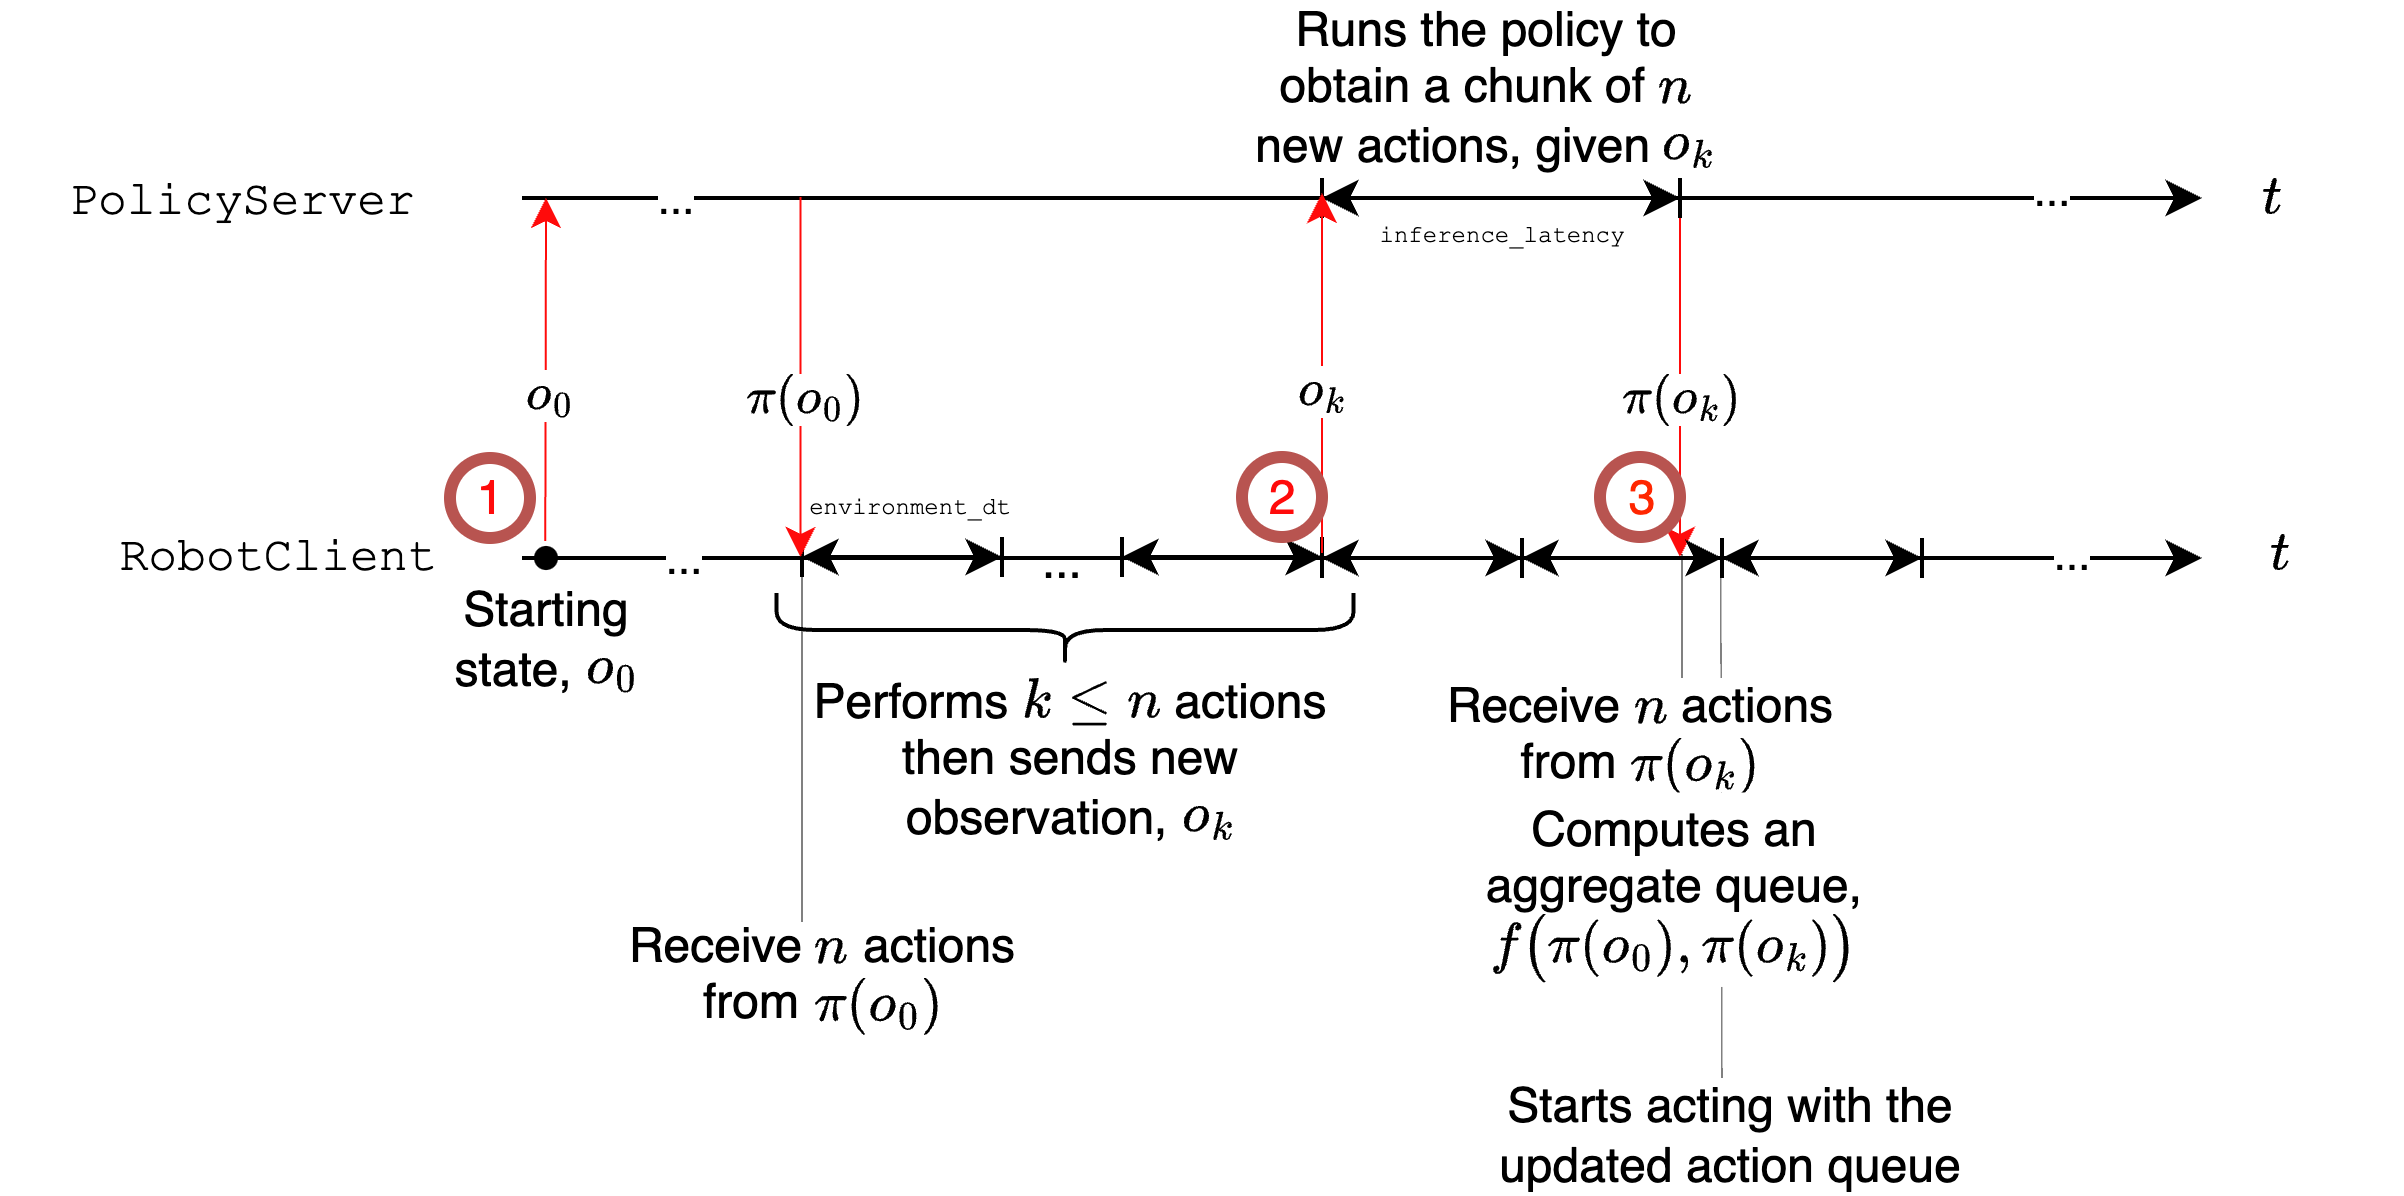
\includegraphics[width=0.9\textwidth]{figures/ch4/ch4-async-inference.png}
        \caption{\textbf{Asynchronous inference}. Illustration of the asynchronous inference stack. Note that the policy can be run on a remote server, possibly with GPUs.}
        \label{fig:ch4-async-inference}
    \end{minipage}
    \vspace{-0.6cm}
\end{figure}

\begin{algorithm}
  \caption{Asynchronous inference control-loop}
  \label{alg:async-inference}
  \begin{algorithmic}[1]
    \State \textbf{Input:} horizon \( T \), chunk size \( H_a \), threshold \( g\in[0,1] \)
    \State \textbf{Init:} capture \( o_0 \); send \( o_0 \) to \textsc{PolicyServer};
           receive \( \actionchunk_0 \gets \pi(o_0) \)
    \For{\( t \) \textbf{to} \( H_a \)}
        \State \( a_t \gets \textsc{PopFront}(\actionchunk_t) \)
        \State \textsc{Execute}(\( a_t \)) \Comment{execute action at step \( t \)}
        \If{\( \tfrac{|\actionchunk_t|}{H_a} < g \)} \Comment{queue below threshold}
            \State capture new observation, \( o_{t+1} \)
            \If{\textsc{NeedsProcessing} \( (o_{t+1}) \) } \Comment{similarity filter, or triggers direct processing}
                \State \texttt{async\_handle} \( \gets \textsc{AsyncInfer}(o_{t+1})\) 
                \Comment{Trigger new chunk prediction (non blocking)}
                \State \( \tilde{\actionchunk}_{t+1} \gets \pi(o_{t+1}) \) \Comment{New queue is predicted with the policy}
                \State \( \actionchunk_{t+1} \gets f(\actionchunk_t,\tilde{\actionchunk}_{t+1}) \) \Comment{aggregate overlaps (if any)}
                
            \EndIf
        \EndIf
        \If {\textsc{NotCompleted}(\texttt{async\_handle})}
            \State \( \actionchunk_{t+1} \gets \actionchunk_t \) \Comment{No update on queue (inference is not over just yet)}
        \EndIf
    \EndFor
  \end{algorithmic}
\end{algorithm}

In practice, \emph{async} inference (1) tightens the control loop by capturing observations more often, eliminating idle gaps at runtime (2) and directly allows to run inference on more powerful computational resources than the ones typically available onboard autonomous robotic platforms.
Algorithmically, one can attain (1) on the \textsc{RobotClient}-side by consuming actions from a readily available queue until a given condition on the number of remaining actions in the queue (\(\vert \actionchunk_t \vert / H_a < g \)) is met. When this condition is triggered, a new observation of the environment is captured and sent to the (possibly remote) \textsc{PolicyServer}. 
To avoid redundant server calls and erratic behavior at runtime observations are compared in joint-space, and near-duplicates are dropped.
Two observations are considered near-duplicates if their distance in joint-space falls under a predetermined threshold, \( d_{\text{lim}} \in \mathbb R_+\).
Importantly, should the queue available to the robot client eventually empty out, the most recent observation is processed regardless of similarity.

Interestingly, the behavior of async inference can be studied analytically. First, let \( \ell \) be a random variable modeling the time needed to receive an action chunk \( \actionchunk \) after sending an observation \( o \), i.e. the sum of (1) the time to send across the observation \( o \) between the \textsc{RobotClient} and \textsc{PolicyServer}, \( t_{C \to S}\) (2) the inference latency on the \textsc{PolicyServer}, \( \ell_S \) and (3) the time to send \( \actionchunk \) between the \textsc{PolicyServer} and \textsc{RobotClient}, \( t_{S \to C} \). Under the (reasonable) assumption of independence, \( \mathbb E [\ell] = \mathbb E[t_{C \to S}] + \mathbb E[\ell_S] + \mathbb E[t_{S \to C}] \), which can be further simplified to \( \mathbb E[\ell] \simeq \mathbb E[\ell_S]  \), assuming communication time is (1) equal in both directions and (2) negligible with respect to the inference latency. Second, let \(\Delta t\) be the environment's control cycle. With a real-world frame-rate of 30 frames-per-second (fps), \(\Delta t=33\text{ms}\). Consequently, exhausted queues at runtime---i.e. being idle awaiting for a new chunk---are avoided for \( g \geq \frac{\mathbb E[\ell_S] / \Delta t}{H_a} \). In this, the action queue threshold \( g \) below which to capture and send a new observation for processing plays a major role relatively to the availability of actions to the \( \textsc{RobotClient} \).

Figure~\ref{fig:ch4-queues} illustrates how the size of the action chunk \(\lvert \actionchunk_t \rvert\) evolves over time for three representative values of \(g\), detailing the following key scenarios:
\begin{itemize}
    \item \textbf{Sequential limit \((g=0)\).} The client drains the entire chunk before forwarding a new observation to the server. During the round-trip latency needed to compute the next chunk, the queue is empty, leaving the robot \emph{incapable of acting}.  This reproduces the behavior of a fully sequential deployment and results in an average of \( \mathbb E[\ell_S] \) idle seconds.
    \item \textbf{Asynchronous inference \((g \in (0,1))\).} Allowing the client to consume a \(1-g\) fraction of its available queue \( \actionchunk_{t-1}\) \emph{before} triggering inference for a new action queue \( \actionchunk_{t} \), computation is amortized while keeping the queue from emptying. The overlap between successive chunks provides a buffer against modeling errors without the full cost of the \(g=1\) regime. The updated queue \( \actionchunk_t\) is obtained aggregating queues on the overlapping timesteps between \( \actionchunk_{t-1}\) and the incoming \(\tilde{\actionchunk}_{t}\).
    \item \textbf{Sync-inference limit \((g=1)\).}  As an extreme case, and in keeping with~\citet{zhaoLearningFineGrainedBimanual2023}, an observation is sent at \emph{every} timestep. The queue is therefore almost always filled, with only a minor saw-tooth due to \(\Delta t/\mathbb E[\ell_s] < 1\). While maximally reactive, this setting incurs one forward pass per control tick and can prove prohibitively expensive on limited hardware. Importantly, because the client is consuming actions while the server computes the next chunk, the available queue never gets entirely filled.
\end{itemize}

\begin{figure}
    \centering
    \begin{minipage}[t]{0.99\textwidth}
        \centering
        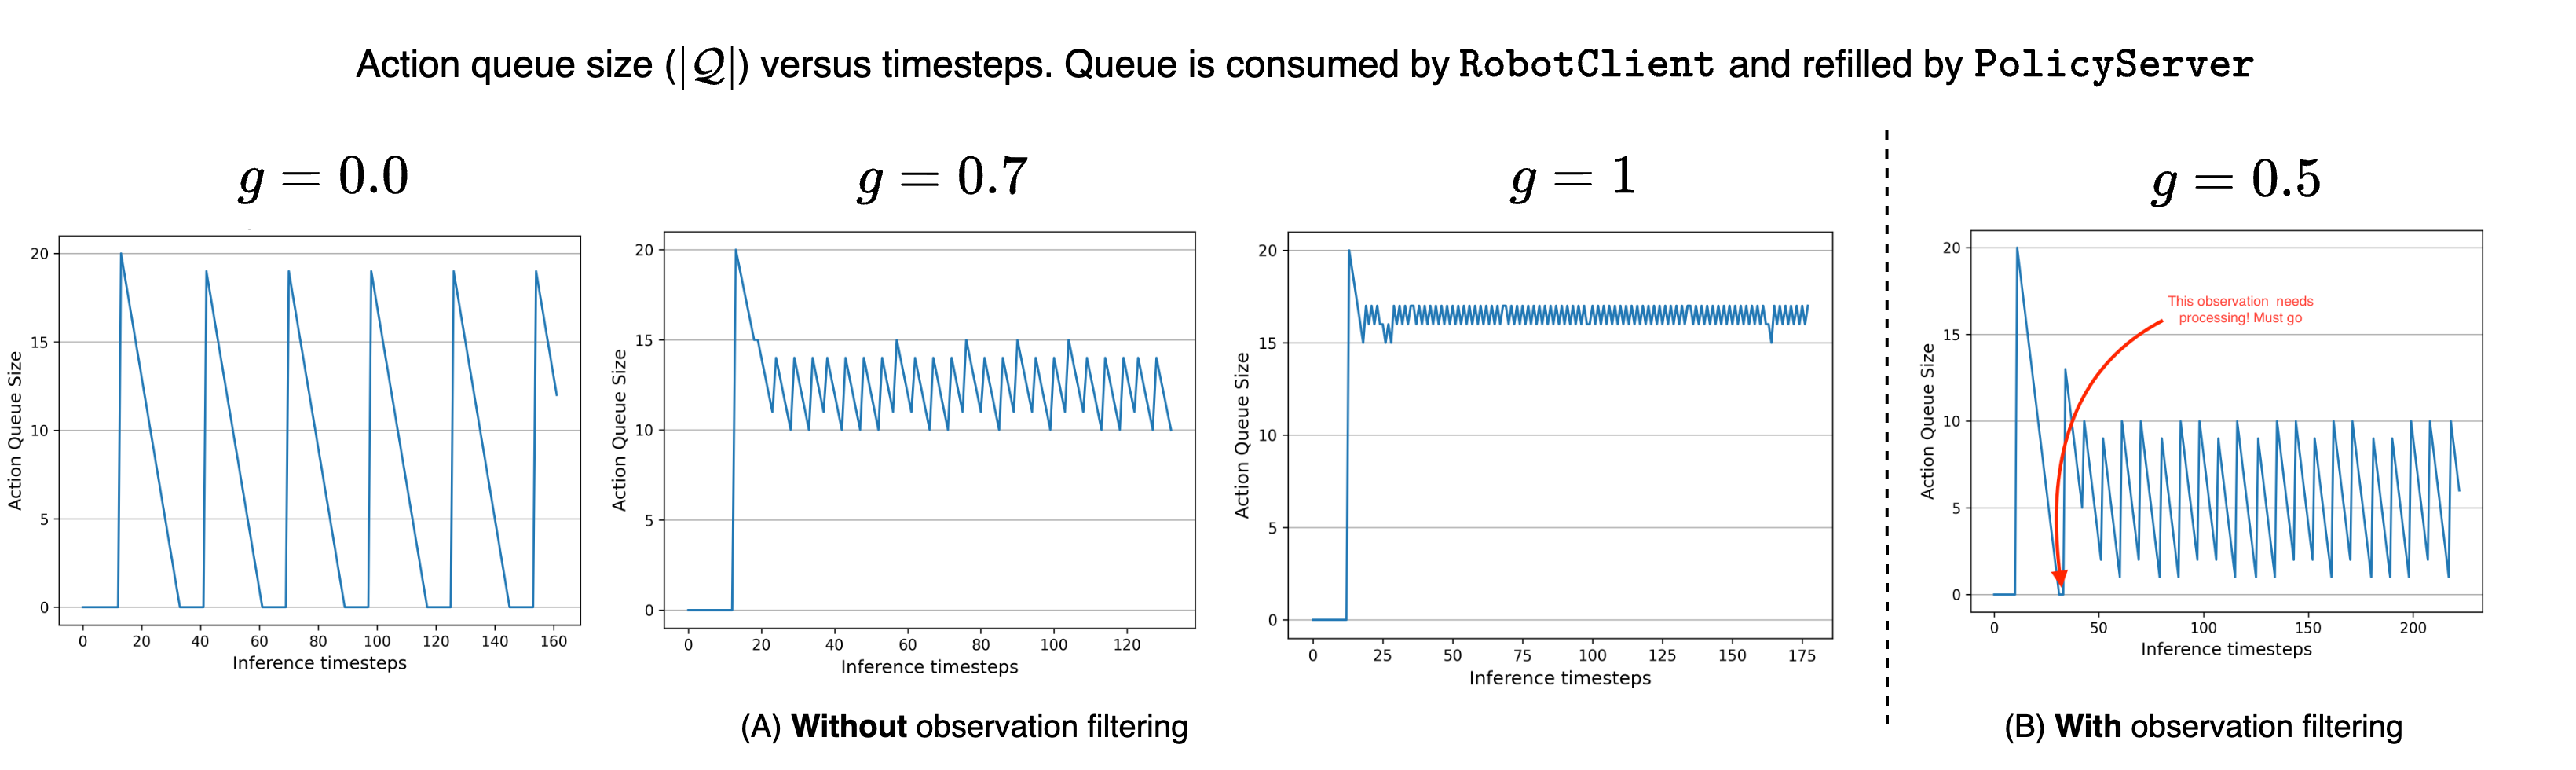
\includegraphics[width=\textwidth]{figures/ch4/ch4-queues.png}
        \caption{Action queue size evolution at runtime for various levels of \( g\) when (A) not filtering out observation based on joint-space similarity and (B) filtering out near-duplicates observation, measuring their similarity in joint-space.}
        \label{fig:ch4-queues}
    \end{minipage}
\end{figure}

Figure~\ref{fig:ch4-queues} emphasizes the trade-off governed by \(g\): small values of \( g \) result in idle periods, whereas \(g\approx 1\) assumes a highly accurate model and pays a significant compute price. 
In practice, choosing \(g\in(0,1)\) allows to strike a balance between reactivity against resource budgets.
If not for the aforementioned similarity filter, the \( \textsc{RobotClient} \) would send observations for processing every \( (1 - g) H_a \cdot \Delta t\) seconds, receiving a new chunk of actions every \( (1 - g) H_a \cdot \Delta t + \mathbb E[\ell_S] \), on average. 
The presence of the filter for observation similarity dilates this processing time, and serves the scope of avoiding the robot stalling due to the queue being constantly integrated with an incoming, nearly identical, action chunk. 
In particular, Figure~\ref{fig:ch4-queues} results in a queue which is filled with incoming actions \emph{unless} near-duplicate observations are filtered out from the processing pipeline. 
For clarity, the red arrow in~\ref{fig:ch4-queues} highlights a timestep where the observation similarity mechanism is bypassed, forcing a (nearly identical) observation to be processed as the queue results empty.

\subsubsection{Code Example: Using Async Inference}

\begin{pbox}[label={ex:spinning-up-server}]{Spinning up a Remote Server}
    \inputminted{python}{snippets/ch4/05_policy_server.py}
\end{pbox}

\begin{pbox}[label={ex:latching-a-robot-client}]{Attaching a Robot Client}
    \inputminted{python}{snippets/ch4/06_robot_client.py}
\end{pbox}